\documentclass[twoside]{book}

% Packages required by doxygen
\usepackage{fixltx2e}
\usepackage{calc}
\usepackage{doxygen}
\usepackage[export]{adjustbox} % also loads graphicx
\usepackage{graphicx}
\usepackage[utf8]{inputenc}
\usepackage{makeidx}
\usepackage{multicol}
\usepackage{multirow}
\PassOptionsToPackage{warn}{textcomp}
\usepackage{textcomp}
\usepackage[nointegrals]{wasysym}
\usepackage[table]{xcolor}

% Font selection
\usepackage[T1]{fontenc}
\usepackage[scaled=.90]{helvet}
\usepackage{courier}
\usepackage{amssymb}
\usepackage{sectsty}
\renewcommand{\familydefault}{\sfdefault}
\allsectionsfont{%
  \fontseries{bc}\selectfont%
  \color{darkgray}%
}
\renewcommand{\DoxyLabelFont}{%
  \fontseries{bc}\selectfont%
  \color{darkgray}%
}
\newcommand{\+}{\discretionary{\mbox{\scriptsize$\hookleftarrow$}}{}{}}

% Page & text layout
\usepackage{geometry}
\geometry{%
  a4paper,%
  top=2.5cm,%
  bottom=2.5cm,%
  left=2.5cm,%
  right=2.5cm%
}
\tolerance=750
\hfuzz=15pt
\hbadness=750
\setlength{\emergencystretch}{15pt}
\setlength{\parindent}{0cm}
\setlength{\parskip}{3ex plus 2ex minus 2ex}
\makeatletter
\renewcommand{\paragraph}{%
  \@startsection{paragraph}{4}{0ex}{-1.0ex}{1.0ex}{%
    \normalfont\normalsize\bfseries\SS@parafont%
  }%
}
\renewcommand{\subparagraph}{%
  \@startsection{subparagraph}{5}{0ex}{-1.0ex}{1.0ex}{%
    \normalfont\normalsize\bfseries\SS@subparafont%
  }%
}
\makeatother

% Headers & footers
\usepackage{fancyhdr}
\pagestyle{fancyplain}
\fancyhead[LE]{\fancyplain{}{\bfseries\thepage}}
\fancyhead[CE]{\fancyplain{}{}}
\fancyhead[RE]{\fancyplain{}{\bfseries\leftmark}}
\fancyhead[LO]{\fancyplain{}{\bfseries\rightmark}}
\fancyhead[CO]{\fancyplain{}{}}
\fancyhead[RO]{\fancyplain{}{\bfseries\thepage}}
\fancyfoot[LE]{\fancyplain{}{}}
\fancyfoot[CE]{\fancyplain{}{}}
\fancyfoot[RE]{\fancyplain{}{\bfseries\scriptsize Generated by Doxygen }}
\fancyfoot[LO]{\fancyplain{}{\bfseries\scriptsize Generated by Doxygen }}
\fancyfoot[CO]{\fancyplain{}{}}
\fancyfoot[RO]{\fancyplain{}{}}
\renewcommand{\footrulewidth}{0.4pt}
\renewcommand{\chaptermark}[1]{%
  \markboth{#1}{}%
}
\renewcommand{\sectionmark}[1]{%
  \markright{\thesection\ #1}%
}

% Indices & bibliography
\usepackage{natbib}
\usepackage[titles]{tocloft}
\setcounter{tocdepth}{3}
\setcounter{secnumdepth}{5}
\makeindex

% Hyperlinks (required, but should be loaded last)
\usepackage{ifpdf}
\ifpdf
  \usepackage[pdftex,pagebackref=true]{hyperref}
\else
  \usepackage[ps2pdf,pagebackref=true]{hyperref}
\fi
\hypersetup{%
  colorlinks=true,%
  linkcolor=blue,%
  citecolor=blue,%
  unicode%
}

% Custom commands
\newcommand{\clearemptydoublepage}{%
  \newpage{\pagestyle{empty}\cleardoublepage}%
}

\usepackage{caption}
\captionsetup{labelsep=space,justification=centering,font={bf},singlelinecheck=off,skip=4pt,position=top}

%===== C O N T E N T S =====

\begin{document}

% Titlepage & ToC
\hypersetup{pageanchor=false,
             bookmarksnumbered=true,
             pdfencoding=unicode
            }
\pagenumbering{roman}
\begin{titlepage}
\vspace*{7cm}
\begin{center}%
{\Large oh\+Captain }\\
\vspace*{1cm}
{\large Generated by Doxygen 1.8.11}\\
\end{center}
\end{titlepage}
\clearemptydoublepage
\tableofcontents
\clearemptydoublepage
\pagenumbering{arabic}
\hypersetup{pageanchor=true}

%--- Begin generated contents ---
\chapter{Namespace Index}
\section{Namespace List}
Here is a list of all namespaces with brief descriptions\+:\begin{DoxyCompactList}
\item\contentsline{section}{\hyperlink{namespaceboost}{boost} }{\pageref{namespaceboost}}{}
\item\contentsline{section}{\hyperlink{namespaceboost_1_1units}{boost\+::units} }{\pageref{namespaceboost_1_1units}}{}
\item\contentsline{section}{\hyperlink{namespaceboost_1_1units_1_1constants}{boost\+::units\+::constants} }{\pageref{namespaceboost_1_1units_1_1constants}}{}
\item\contentsline{section}{\hyperlink{namespaceboost_1_1units_1_1literals}{boost\+::units\+::literals} }{\pageref{namespaceboost_1_1units_1_1literals}}{}
\item\contentsline{section}{\hyperlink{namespaceo_cpt}{o\+Cpt} }{\pageref{namespaceo_cpt}}{}
\item\contentsline{section}{\hyperlink{namespaceo_cpt_1_1components}{o\+Cpt\+::components} }{\pageref{namespaceo_cpt_1_1components}}{}
\item\contentsline{section}{\hyperlink{namespaceo_cpt_1_1components_1_1comm}{o\+Cpt\+::components\+::comm} }{\pageref{namespaceo_cpt_1_1components_1_1comm}}{}
\item\contentsline{section}{\hyperlink{namespaceo_cpt_1_1components_1_1controller}{o\+Cpt\+::components\+::controller} }{\pageref{namespaceo_cpt_1_1components_1_1controller}}{}
\item\contentsline{section}{\hyperlink{namespaceo_cpt_1_1components_1_1sensors}{o\+Cpt\+::components\+::sensors} }{\pageref{namespaceo_cpt_1_1components_1_1sensors}}{}
\item\contentsline{section}{\hyperlink{namespaceo_cpt_1_1protocol}{o\+Cpt\+::protocol} }{\pageref{namespaceo_cpt_1_1protocol}}{}
\item\contentsline{section}{\hyperlink{namespaceo_cpt_1_1vessels}{o\+Cpt\+::vessels} }{\pageref{namespaceo_cpt_1_1vessels}}{}
\end{DoxyCompactList}

\chapter{Hierarchical Index}
\section{Class Hierarchy}
This inheritance list is sorted roughly, but not completely, alphabetically\+:\begin{DoxyCompactList}
\item \contentsline{section}{o\+Cpt\+:\+:World\+:\+:Location\+:\+:coordinate}{\pageref{structo_cpt_1_1_world_1_1_location_1_1coordinate}}{}
\item enable\+\_\+shared\+\_\+from\+\_\+this\begin{DoxyCompactList}
\item \contentsline{section}{o\+Cpt\+:\+:i\+Boatswain}{\pageref{classo_cpt_1_1i_boatswain}}{}
\begin{DoxyCompactList}
\item \contentsline{section}{o\+Cpt\+:\+:Boatswain}{\pageref{classo_cpt_1_1_boatswain}}{}
\end{DoxyCompactList}
\end{DoxyCompactList}
\item exception\begin{DoxyCompactList}
\item \contentsline{section}{o\+Cpt\+:\+:o\+Cpt\+Exception}{\pageref{classo_cpt_1_1o_cpt_exception}}{}
\end{DoxyCompactList}
\item \contentsline{section}{o\+Cpt\+:\+:World\+:\+:Location\+:\+:gps\+Point}{\pageref{structo_cpt_1_1_world_1_1_location_1_1gps_point}}{}
\item \contentsline{section}{o\+Cpt\+:\+:i\+Actuator}{\pageref{classo_cpt_1_1i_actuator}}{}
\begin{DoxyCompactList}
\item \contentsline{section}{o\+Cpt\+:\+:Actuator}{\pageref{classo_cpt_1_1_actuator}}{}
\end{DoxyCompactList}
\item \contentsline{section}{o\+Cpt\+:\+:i\+Captain}{\pageref{classo_cpt_1_1i_captain}}{}
\begin{DoxyCompactList}
\item \contentsline{section}{o\+Cpt\+:\+:Captain}{\pageref{classo_cpt_1_1_captain}}{}
\end{DoxyCompactList}
\item \contentsline{section}{o\+Cpt\+:\+:i\+Comm}{\pageref{classo_cpt_1_1i_comm}}{}
\begin{DoxyCompactList}
\item \contentsline{section}{o\+Cpt\+:\+:Lo\+Ra}{\pageref{classo_cpt_1_1_lo_ra}}{}
\begin{DoxyCompactList}
\item \contentsline{section}{o\+Cpt\+:\+:components\+:\+:comm\+:\+:Lo\+Ra\+\_\+\+R\+N2483}{\pageref{classo_cpt_1_1components_1_1comm_1_1_lo_ra___r_n2483}}{}
\end{DoxyCompactList}
\end{DoxyCompactList}
\item \contentsline{section}{o\+Cpt\+:\+:i\+Controller}{\pageref{classo_cpt_1_1i_controller}}{}
\begin{DoxyCompactList}
\item \contentsline{section}{o\+Cpt\+:\+:A\+RM}{\pageref{classo_cpt_1_1_a_r_m}}{}
\begin{DoxyCompactList}
\item \contentsline{section}{o\+Cpt\+:\+:components\+:\+:controller\+:\+:B\+BB}{\pageref{classo_cpt_1_1components_1_1controller_1_1_b_b_b}}{}
\end{DoxyCompactList}
\end{DoxyCompactList}
\item \contentsline{section}{o\+Cpt\+:\+:i\+Sensor}{\pageref{classo_cpt_1_1i_sensor}}{}
\begin{DoxyCompactList}
\item \contentsline{section}{o\+Cpt\+:\+:Sensor}{\pageref{classo_cpt_1_1_sensor}}{}
\begin{DoxyCompactList}
\item \contentsline{section}{o\+Cpt\+:\+:components\+:\+:sensors\+:\+:Gps}{\pageref{classo_cpt_1_1components_1_1sensors_1_1_gps}}{}
\item \contentsline{section}{o\+Cpt\+:\+:components\+:\+:sensors\+:\+:Kalman\+I\+MU}{\pageref{classo_cpt_1_1components_1_1sensors_1_1_kalman_i_m_u}}{}
\item \contentsline{section}{o\+Cpt\+:\+:components\+:\+:sensors\+:\+:P\+T100}{\pageref{classo_cpt_1_1components_1_1sensors_1_1_p_t100}}{}
\item \contentsline{section}{o\+Cpt\+:\+:components\+:\+:sensors\+:\+:Razor}{\pageref{classo_cpt_1_1components_1_1sensors_1_1_razor}}{}
\end{DoxyCompactList}
\end{DoxyCompactList}
\item \contentsline{section}{o\+Cpt\+:\+:i\+Task}{\pageref{classo_cpt_1_1i_task}}{}
\begin{DoxyCompactList}
\item \contentsline{section}{o\+Cpt\+:\+:Task}{\pageref{classo_cpt_1_1_task}}{}
\begin{DoxyCompactList}
\item \contentsline{section}{o\+Cpt\+:\+:Route\+Task}{\pageref{classo_cpt_1_1_route_task}}{}
\begin{DoxyCompactList}
\item \contentsline{section}{o\+Cpt\+:\+:Coverage\+Path\+Task}{\pageref{classo_cpt_1_1_coverage_path_task}}{}
\item \contentsline{section}{o\+Cpt\+:\+:Follow\+Task}{\pageref{classo_cpt_1_1_follow_task}}{}
\item \contentsline{section}{o\+Cpt\+:\+:Path\+Task}{\pageref{classo_cpt_1_1_path_task}}{}
\end{DoxyCompactList}
\item \contentsline{section}{o\+Cpt\+:\+:Work\+Task}{\pageref{classo_cpt_1_1_work_task}}{}
\begin{DoxyCompactList}
\item \contentsline{section}{o\+Cpt\+:\+:Actuator\+Task}{\pageref{classo_cpt_1_1_actuator_task}}{}
\item \contentsline{section}{o\+Cpt\+:\+:Communication\+Task}{\pageref{classo_cpt_1_1_communication_task}}{}
\item \contentsline{section}{o\+Cpt\+:\+:Dredge\+Task}{\pageref{classo_cpt_1_1_dredge_task}}{}
\item \contentsline{section}{o\+Cpt\+:\+:Log\+Task}{\pageref{classo_cpt_1_1_log_task}}{}
\item \contentsline{section}{o\+Cpt\+:\+:Sensor\+Task}{\pageref{classo_cpt_1_1_sensor_task}}{}
\end{DoxyCompactList}
\end{DoxyCompactList}
\end{DoxyCompactList}
\item \contentsline{section}{o\+Cpt\+:\+:i\+Vessel}{\pageref{classo_cpt_1_1i_vessel}}{}
\begin{DoxyCompactList}
\item \contentsline{section}{o\+Cpt\+:\+:Vessel}{\pageref{classo_cpt_1_1_vessel}}{}
\begin{DoxyCompactList}
\item \contentsline{section}{o\+Cpt\+:\+:vessels\+:\+:Meetcatamaran}{\pageref{classo_cpt_1_1vessels_1_1_meetcatamaran}}{}
\end{DoxyCompactList}
\end{DoxyCompactList}
\item Linearized\+Measurement\+Model\begin{DoxyCompactList}
\item \contentsline{section}{o\+Cpt\+:\+:components\+:\+:sensors\+:\+:Orientation\+Measurement\+Model\+Kalman\+I\+MU$<$ T, Covariance\+Base $>$}{\pageref{classo_cpt_1_1components_1_1sensors_1_1_orientation_measurement_model_kalman_i_m_u}}{}
\item \contentsline{section}{o\+Cpt\+:\+:components\+:\+:sensors\+:\+:Position\+Measurement\+Model\+Kalman\+I\+MU$<$ T, Covariance\+Base $>$}{\pageref{classo_cpt_1_1components_1_1sensors_1_1_position_measurement_model_kalman_i_m_u}}{}
\end{DoxyCompactList}
\item Linearized\+System\+Model\begin{DoxyCompactList}
\item \contentsline{section}{o\+Cpt\+:\+:components\+:\+:sensors\+:\+:System\+Model\+Kalman\+I\+MU$<$ T, Covariance\+Base $>$}{\pageref{classo_cpt_1_1components_1_1sensors_1_1_system_model_kalman_i_m_u}}{}
\end{DoxyCompactList}
\item \contentsline{section}{o\+Cpt\+:\+:World\+:\+:Location}{\pageref{classo_cpt_1_1_world_1_1_location}}{}
\item \contentsline{section}{o\+Cpt\+:\+:World\+:\+:Time\+:\+:Log$<$ T $>$}{\pageref{classo_cpt_1_1_world_1_1_time_1_1_log}}{}
\item \contentsline{section}{o\+Cpt\+:\+:i\+Comm\+:\+:Message}{\pageref{structo_cpt_1_1i_comm_1_1_message}}{}
\item \contentsline{section}{o\+Cpt\+:\+:components\+:\+:sensors\+:\+:Razor\+:\+:Return\+Value}{\pageref{structo_cpt_1_1components_1_1sensors_1_1_razor_1_1_return_value}}{}
\item \contentsline{section}{o\+Cpt\+:\+:components\+:\+:sensors\+:\+:Kalman\+I\+MU\+:\+:Return\+Value}{\pageref{structo_cpt_1_1components_1_1sensors_1_1_kalman_i_m_u_1_1_return_value}}{}
\item \contentsline{section}{o\+Cpt\+:\+:World\+:\+:Location\+:\+:Route\+Point}{\pageref{structo_cpt_1_1_world_1_1_location_1_1_route_point}}{}
\item \contentsline{section}{o\+Cpt\+:\+:i\+Sensor\+:\+:State}{\pageref{structo_cpt_1_1i_sensor_1_1_state}}{}
\item \contentsline{section}{o\+Cpt\+:\+:i\+Task\+:\+:Status}{\pageref{classo_cpt_1_1i_task_1_1_status}}{}
\item \contentsline{section}{o\+Cpt\+:\+:World\+:\+:Time}{\pageref{classo_cpt_1_1_world_1_1_time}}{}
\item \contentsline{section}{o\+Cpt\+:\+:protocol\+:\+:userspace}{\pageref{classo_cpt_1_1protocol_1_1userspace}}{}
\begin{DoxyCompactList}
\item \contentsline{section}{o\+Cpt\+:\+:protocol\+:\+:adc}{\pageref{classo_cpt_1_1protocol_1_1adc}}{}
\item \contentsline{section}{o\+Cpt\+:\+:protocol\+:\+:gpio}{\pageref{classo_cpt_1_1protocol_1_1gpio}}{}
\item \contentsline{section}{o\+Cpt\+:\+:protocol\+:\+:Serial}{\pageref{classo_cpt_1_1protocol_1_1_serial}}{}
\end{DoxyCompactList}
\item Vector\begin{DoxyCompactList}
\item \contentsline{section}{o\+Cpt\+:\+:components\+:\+:sensors\+:\+:Control\+Kalman\+I\+MU$<$ T $>$}{\pageref{classo_cpt_1_1components_1_1sensors_1_1_control_kalman_i_m_u}}{}
\item \contentsline{section}{o\+Cpt\+:\+:components\+:\+:sensors\+:\+:Orientation\+Measurement\+Kalman\+I\+MU$<$ T $>$}{\pageref{classo_cpt_1_1components_1_1sensors_1_1_orientation_measurement_kalman_i_m_u}}{}
\item \contentsline{section}{o\+Cpt\+:\+:components\+:\+:sensors\+:\+:Position\+Measurement\+Kalman\+I\+MU$<$ T $>$}{\pageref{classo_cpt_1_1components_1_1sensors_1_1_position_measurement_kalman_i_m_u}}{}
\item \contentsline{section}{o\+Cpt\+:\+:components\+:\+:sensors\+:\+:State\+Kalman\+I\+MU$<$ T $>$}{\pageref{classo_cpt_1_1components_1_1sensors_1_1_state_kalman_i_m_u}}{}
\end{DoxyCompactList}
\item \contentsline{section}{o\+Cpt\+:\+:World}{\pageref{classo_cpt_1_1_world}}{}
\end{DoxyCompactList}

\chapter{Class Index}
\section{Class List}
Here are the classes, structs, unions and interfaces with brief descriptions\+:\begin{DoxyCompactList}
\item\contentsline{section}{\hyperlink{classo_cpt_1_1_actuator}{o\+Cpt\+::\+Actuator} }{\pageref{classo_cpt_1_1_actuator}}{}
\item\contentsline{section}{\hyperlink{classo_cpt_1_1_actuator_task}{o\+Cpt\+::\+Actuator\+Task} }{\pageref{classo_cpt_1_1_actuator_task}}{}
\item\contentsline{section}{\hyperlink{classo_cpt_1_1protocol_1_1adc}{o\+Cpt\+::protocol\+::adc} }{\pageref{classo_cpt_1_1protocol_1_1adc}}{}
\item\contentsline{section}{\hyperlink{classo_cpt_1_1_a_r_m}{o\+Cpt\+::\+A\+RM} }{\pageref{classo_cpt_1_1_a_r_m}}{}
\item\contentsline{section}{\hyperlink{classo_cpt_1_1components_1_1controller_1_1_b_b_b}{o\+Cpt\+::components\+::controller\+::\+B\+BB} }{\pageref{classo_cpt_1_1components_1_1controller_1_1_b_b_b}}{}
\item\contentsline{section}{\hyperlink{classo_cpt_1_1_boatswain}{o\+Cpt\+::\+Boatswain} }{\pageref{classo_cpt_1_1_boatswain}}{}
\item\contentsline{section}{\hyperlink{classo_cpt_1_1_captain}{o\+Cpt\+::\+Captain} }{\pageref{classo_cpt_1_1_captain}}{}
\item\contentsline{section}{\hyperlink{classo_cpt_1_1_communication_task}{o\+Cpt\+::\+Communication\+Task} }{\pageref{classo_cpt_1_1_communication_task}}{}
\item\contentsline{section}{\hyperlink{structo_cpt_1_1_world_1_1_location_1_1coordinate}{o\+Cpt\+::\+World\+::\+Location\+::coordinate} }{\pageref{structo_cpt_1_1_world_1_1_location_1_1coordinate}}{}
\item\contentsline{section}{\hyperlink{classo_cpt_1_1_coverage_path_task}{o\+Cpt\+::\+Coverage\+Path\+Task} \\*An object representing a coverage path task }{\pageref{classo_cpt_1_1_coverage_path_task}}{}
\item\contentsline{section}{\hyperlink{classo_cpt_1_1_dredge_task}{o\+Cpt\+::\+Dredge\+Task} \\*An Object representing a dredging task }{\pageref{classo_cpt_1_1_dredge_task}}{}
\item\contentsline{section}{\hyperlink{classo_cpt_1_1_follow_task}{o\+Cpt\+::\+Follow\+Task} \\*An object representing a follow the target task }{\pageref{classo_cpt_1_1_follow_task}}{}
\item\contentsline{section}{\hyperlink{classo_cpt_1_1protocol_1_1gpio}{o\+Cpt\+::protocol\+::gpio} }{\pageref{classo_cpt_1_1protocol_1_1gpio}}{}
\item\contentsline{section}{\hyperlink{classo_cpt_1_1components_1_1sensors_1_1_gps}{o\+Cpt\+::components\+::sensors\+::\+Gps} }{\pageref{classo_cpt_1_1components_1_1sensors_1_1_gps}}{}
\item\contentsline{section}{\hyperlink{structo_cpt_1_1_world_1_1_location_1_1gps_point}{o\+Cpt\+::\+World\+::\+Location\+::gps\+Point} }{\pageref{structo_cpt_1_1_world_1_1_location_1_1gps_point}}{}
\item\contentsline{section}{\hyperlink{classo_cpt_1_1i_actuator}{o\+Cpt\+::i\+Actuator} }{\pageref{classo_cpt_1_1i_actuator}}{}
\item\contentsline{section}{\hyperlink{classo_cpt_1_1i_boatswain}{o\+Cpt\+::i\+Boatswain} }{\pageref{classo_cpt_1_1i_boatswain}}{}
\item\contentsline{section}{\hyperlink{classo_cpt_1_1i_captain}{o\+Cpt\+::i\+Captain} }{\pageref{classo_cpt_1_1i_captain}}{}
\item\contentsline{section}{\hyperlink{classo_cpt_1_1i_comm}{o\+Cpt\+::i\+Comm} }{\pageref{classo_cpt_1_1i_comm}}{}
\item\contentsline{section}{\hyperlink{classo_cpt_1_1i_controller}{o\+Cpt\+::i\+Controller} }{\pageref{classo_cpt_1_1i_controller}}{}
\item\contentsline{section}{\hyperlink{classo_cpt_1_1i_sensor}{o\+Cpt\+::i\+Sensor} }{\pageref{classo_cpt_1_1i_sensor}}{}
\item\contentsline{section}{\hyperlink{classo_cpt_1_1i_task}{o\+Cpt\+::i\+Task} \\*\hyperlink{classo_cpt_1_1_task}{Task} interface, all tasks need to adhere to this structure }{\pageref{classo_cpt_1_1i_task}}{}
\item\contentsline{section}{\hyperlink{classo_cpt_1_1i_vessel}{o\+Cpt\+::i\+Vessel} }{\pageref{classo_cpt_1_1i_vessel}}{}
\item\contentsline{section}{\hyperlink{classo_cpt_1_1_world_1_1_location}{o\+Cpt\+::\+World\+::\+Location} }{\pageref{classo_cpt_1_1_world_1_1_location}}{}
\item\contentsline{section}{\hyperlink{classo_cpt_1_1_world_1_1_time_1_1_log}{o\+Cpt\+::\+World\+::\+Time\+::\+Log$<$ T $>$} }{\pageref{classo_cpt_1_1_world_1_1_time_1_1_log}}{}
\item\contentsline{section}{\hyperlink{classo_cpt_1_1_log_task}{o\+Cpt\+::\+Log\+Task} \\*An Object representing a data logging task }{\pageref{classo_cpt_1_1_log_task}}{}
\item\contentsline{section}{\hyperlink{classo_cpt_1_1_lo_ra}{o\+Cpt\+::\+Lo\+Ra} }{\pageref{classo_cpt_1_1_lo_ra}}{}
\item\contentsline{section}{\hyperlink{classo_cpt_1_1components_1_1comm_1_1_lo_ra___r_n2483}{o\+Cpt\+::components\+::comm\+::\+Lo\+Ra\+\_\+\+R\+N2483} }{\pageref{classo_cpt_1_1components_1_1comm_1_1_lo_ra___r_n2483}}{}
\item\contentsline{section}{\hyperlink{classo_cpt_1_1vessels_1_1_meetcatamaran}{o\+Cpt\+::vessels\+::\+Meetcatamaran} }{\pageref{classo_cpt_1_1vessels_1_1_meetcatamaran}}{}
\item\contentsline{section}{\hyperlink{structo_cpt_1_1i_comm_1_1_message}{o\+Cpt\+::i\+Comm\+::\+Message} }{\pageref{structo_cpt_1_1i_comm_1_1_message}}{}
\item\contentsline{section}{\hyperlink{classo_cpt_1_1o_cpt_exception}{o\+Cpt\+::o\+Cpt\+Exception} }{\pageref{classo_cpt_1_1o_cpt_exception}}{}
\item\contentsline{section}{\hyperlink{classo_cpt_1_1_path_task}{o\+Cpt\+::\+Path\+Task} \\*An object representing a normal A to B type of path planning }{\pageref{classo_cpt_1_1_path_task}}{}
\item\contentsline{section}{\hyperlink{classo_cpt_1_1components_1_1sensors_1_1_p_t100}{o\+Cpt\+::components\+::sensors\+::\+P\+T100} }{\pageref{classo_cpt_1_1components_1_1sensors_1_1_p_t100}}{}
\item\contentsline{section}{\hyperlink{classo_cpt_1_1components_1_1sensors_1_1_razor}{o\+Cpt\+::components\+::sensors\+::\+Razor} }{\pageref{classo_cpt_1_1components_1_1sensors_1_1_razor}}{}
\item\contentsline{section}{\hyperlink{structo_cpt_1_1components_1_1sensors_1_1_razor_1_1_return_value}{o\+Cpt\+::components\+::sensors\+::\+Razor\+::\+Return\+Value} }{\pageref{structo_cpt_1_1components_1_1sensors_1_1_razor_1_1_return_value}}{}
\item\contentsline{section}{\hyperlink{structo_cpt_1_1_world_1_1_location_1_1_route_point}{o\+Cpt\+::\+World\+::\+Location\+::\+Route\+Point} }{\pageref{structo_cpt_1_1_world_1_1_location_1_1_route_point}}{}
\item\contentsline{section}{\hyperlink{classo_cpt_1_1_route_task}{o\+Cpt\+::\+Route\+Task} }{\pageref{classo_cpt_1_1_route_task}}{}
\item\contentsline{section}{\hyperlink{classo_cpt_1_1_sensor}{o\+Cpt\+::\+Sensor} }{\pageref{classo_cpt_1_1_sensor}}{}
\item\contentsline{section}{\hyperlink{classo_cpt_1_1_sensor_task}{o\+Cpt\+::\+Sensor\+Task} }{\pageref{classo_cpt_1_1_sensor_task}}{}
\item\contentsline{section}{\hyperlink{classo_cpt_1_1protocol_1_1_serial}{o\+Cpt\+::protocol\+::\+Serial} }{\pageref{classo_cpt_1_1protocol_1_1_serial}}{}
\item\contentsline{section}{\hyperlink{structo_cpt_1_1i_sensor_1_1_state}{o\+Cpt\+::i\+Sensor\+::\+State} }{\pageref{structo_cpt_1_1i_sensor_1_1_state}}{}
\item\contentsline{section}{\hyperlink{classo_cpt_1_1i_task_1_1_status}{o\+Cpt\+::i\+Task\+::\+Status} }{\pageref{classo_cpt_1_1i_task_1_1_status}}{}
\item\contentsline{section}{\hyperlink{classo_cpt_1_1_task}{o\+Cpt\+::\+Task} }{\pageref{classo_cpt_1_1_task}}{}
\item\contentsline{section}{\hyperlink{classo_cpt_1_1_world_1_1_time}{o\+Cpt\+::\+World\+::\+Time} }{\pageref{classo_cpt_1_1_world_1_1_time}}{}
\item\contentsline{section}{\hyperlink{classo_cpt_1_1protocol_1_1userspace}{o\+Cpt\+::protocol\+::userspace} }{\pageref{classo_cpt_1_1protocol_1_1userspace}}{}
\item\contentsline{section}{\hyperlink{classo_cpt_1_1_vessel}{o\+Cpt\+::\+Vessel} }{\pageref{classo_cpt_1_1_vessel}}{}
\item\contentsline{section}{\hyperlink{classo_cpt_1_1_work_task}{o\+Cpt\+::\+Work\+Task} }{\pageref{classo_cpt_1_1_work_task}}{}
\item\contentsline{section}{\hyperlink{classo_cpt_1_1_world}{o\+Cpt\+::\+World} }{\pageref{classo_cpt_1_1_world}}{}
\end{DoxyCompactList}

\chapter{File Index}
\section{File List}
Here is a list of all files with brief descriptions\+:\begin{DoxyCompactList}
\item\contentsline{section}{include/\+Communication/\hyperlink{_lo_ra___r_n2483_8h}{Lo\+Ra\+\_\+\+R\+N2483.\+h} }{\pageref{_lo_ra___r_n2483_8h}}{}
\item\contentsline{section}{include/\+Controllers/\hyperlink{_beaglebone_black_8h}{Beaglebone\+Black.\+h} }{\pageref{_beaglebone_black_8h}}{}
\item\contentsline{section}{include/\+Core/\hyperlink{_actuator_8h}{Actuator.\+h} }{\pageref{_actuator_8h}}{}
\item\contentsline{section}{include/\+Core/\hyperlink{_boatswain_8h}{Boatswain.\+h} }{\pageref{_boatswain_8h}}{}
\item\contentsline{section}{include/\+Core/\hyperlink{_captain_8h}{Captain.\+h} }{\pageref{_captain_8h}}{}
\item\contentsline{section}{include/\+Core/\hyperlink{_communication_8h}{Communication.\+h} }{\pageref{_communication_8h}}{}
\item\contentsline{section}{include/\+Core/\hyperlink{_controller_8h}{Controller.\+h} }{\pageref{_controller_8h}}{}
\item\contentsline{section}{include/\+Core/\hyperlink{_exception_8h}{Exception.\+h} }{\pageref{_exception_8h}}{}
\item\contentsline{section}{include/\+Core/\hyperlink{_sensor_8h}{Sensor.\+h} }{\pageref{_sensor_8h}}{}
\item\contentsline{section}{include/\+Core/\hyperlink{_task_8h}{Task.\+h} }{\pageref{_task_8h}}{}
\item\contentsline{section}{include/\+Core/\hyperlink{_vessel_8h}{Vessel.\+h} }{\pageref{_vessel_8h}}{}
\item\contentsline{section}{include/\+Core/\hyperlink{_world_8h}{World.\+h} }{\pageref{_world_8h}}{}
\item\contentsline{section}{include/\+Sensors/\hyperlink{_gps_8h}{Gps.\+h} }{\pageref{_gps_8h}}{}
\item\contentsline{section}{include/\+Sensors/\hyperlink{_p_t100_8h}{P\+T100.\+h} }{\pageref{_p_t100_8h}}{}
\item\contentsline{section}{include/\+Sensors/\hyperlink{_razor_8h}{Razor.\+h} }{\pageref{_razor_8h}}{}
\item\contentsline{section}{include/\+Vessels/\hyperlink{_meetcatamaran_8h}{Meetcatamaran.\+h} }{\pageref{_meetcatamaran_8h}}{}
\item\contentsline{section}{src/\+Communication/\hyperlink{_lo_ra___r_n2483_8cpp}{Lo\+Ra\+\_\+\+R\+N2483.\+cpp} }{\pageref{_lo_ra___r_n2483_8cpp}}{}
\item\contentsline{section}{src/\+Controllers/\hyperlink{_beaglebone_black_8cpp}{Beaglebone\+Black.\+cpp} }{\pageref{_beaglebone_black_8cpp}}{}
\item\contentsline{section}{src/\+Core/\hyperlink{_actuator_8cpp}{Actuator.\+cpp} }{\pageref{_actuator_8cpp}}{}
\item\contentsline{section}{src/\+Core/\hyperlink{_boatswain_8cpp}{Boatswain.\+cpp} }{\pageref{_boatswain_8cpp}}{}
\item\contentsline{section}{src/\+Core/\hyperlink{_captain_8cpp}{Captain.\+cpp} }{\pageref{_captain_8cpp}}{}
\item\contentsline{section}{src/\+Core/\hyperlink{_communication_8cpp}{Communication.\+cpp} }{\pageref{_communication_8cpp}}{}
\item\contentsline{section}{src/\+Core/\hyperlink{_controller_8cpp}{Controller.\+cpp} }{\pageref{_controller_8cpp}}{}
\item\contentsline{section}{src/\+Core/\hyperlink{_sensor_8cpp}{Sensor.\+cpp} }{\pageref{_sensor_8cpp}}{}
\item\contentsline{section}{src/\+Core/\hyperlink{_task_8cpp}{Task.\+cpp} }{\pageref{_task_8cpp}}{}
\item\contentsline{section}{src/\+Core/\hyperlink{_vessel_8cpp}{Vessel.\+cpp} }{\pageref{_vessel_8cpp}}{}
\item\contentsline{section}{src/\+Core/\hyperlink{_world_8cpp}{World.\+cpp} }{\pageref{_world_8cpp}}{}
\item\contentsline{section}{src/\+Sensors/\hyperlink{_gps_8cpp}{Gps.\+cpp} }{\pageref{_gps_8cpp}}{}
\item\contentsline{section}{src/\+Sensors/\hyperlink{_p_t100_8cpp}{P\+T100.\+cpp} }{\pageref{_p_t100_8cpp}}{}
\item\contentsline{section}{src/\+Sensors/\hyperlink{_razor_8cpp}{Razor.\+cpp} }{\pageref{_razor_8cpp}}{}
\item\contentsline{section}{src/\+Vessels/\hyperlink{_meetcatamaran_8cpp}{Meetcatamaran.\+cpp} }{\pageref{_meetcatamaran_8cpp}}{}
\end{DoxyCompactList}

\chapter{Namespace Documentation}
\hypertarget{namespaceo_cpt}{}\section{o\+Cpt Namespace Reference}
\label{namespaceo_cpt}\index{o\+Cpt@{o\+Cpt}}
\subsection*{Classes}
\begin{DoxyCompactItemize}
\item 
class \hyperlink{classo_cpt_1_1_coverage_path_task}{Coverage\+Path\+Task}
\begin{DoxyCompactList}\small\item\em An object representing a coverage path task. \end{DoxyCompactList}\item 
class \hyperlink{classo_cpt_1_1_dredge_task}{Dredge\+Task}
\begin{DoxyCompactList}\small\item\em An Object representing a dredging task. \end{DoxyCompactList}\item 
class \hyperlink{classo_cpt_1_1_follow_task}{Follow\+Task}
\begin{DoxyCompactList}\small\item\em An object representing a follow the target task. \end{DoxyCompactList}\item 
class \hyperlink{classo_cpt_1_1i_task}{i\+Task}
\begin{DoxyCompactList}\small\item\em \hyperlink{classo_cpt_1_1_task}{Task} interface, all tasks need to adhere to this structure. \end{DoxyCompactList}\item 
class \hyperlink{classo_cpt_1_1_log_task}{Log\+Task}
\begin{DoxyCompactList}\small\item\em An Object representing a data logging task. \end{DoxyCompactList}\item 
class \hyperlink{classo_cpt_1_1_path_task}{Path\+Task}
\begin{DoxyCompactList}\small\item\em An object representing a normal A to B type of path planning. \end{DoxyCompactList}\item 
class \hyperlink{classo_cpt_1_1_route_task}{Route\+Task}
\item 
class \hyperlink{classo_cpt_1_1_task}{Task}
\item 
class \hyperlink{classo_cpt_1_1_work_task}{Work\+Task}
\end{DoxyCompactItemize}

\chapter{Class Documentation}
\hypertarget{classo_cpt_1_1_coverage_path_task}{}\section{o\+Cpt\+:\+:Coverage\+Path\+Task Class Reference}
\label{classo_cpt_1_1_coverage_path_task}\index{o\+Cpt\+::\+Coverage\+Path\+Task@{o\+Cpt\+::\+Coverage\+Path\+Task}}


An object representing a coverage path task.  




{\ttfamily \#include $<$Task.\+h$>$}

Inheritance diagram for o\+Cpt\+:\+:Coverage\+Path\+Task\+:\begin{figure}[H]
\begin{center}
\leavevmode
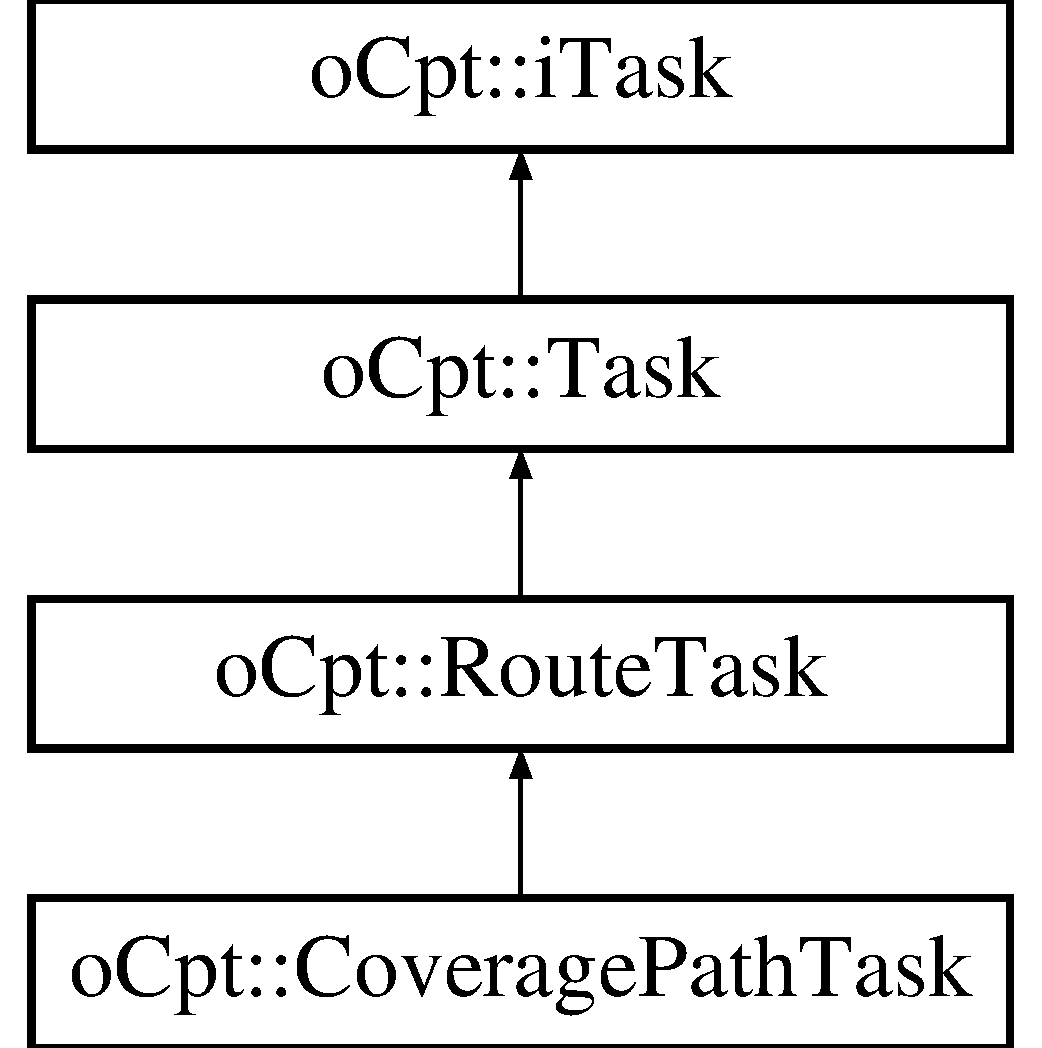
\includegraphics[height=4.000000cm]{classo_cpt_1_1_coverage_path_task}
\end{center}
\end{figure}
\subsection*{Public Member Functions}
\begin{DoxyCompactItemize}
\item 
\hyperlink{classo_cpt_1_1_coverage_path_task_abfdaef848200d9ad4173692cde984ca8}{Coverage\+Path\+Task} ()
\item 
virtual \hyperlink{classo_cpt_1_1_coverage_path_task_a8773343bb232c3a22b8ec6acf483bee1}{$\sim$\+Coverage\+Path\+Task} ()
\end{DoxyCompactItemize}
\subsection*{Additional Inherited Members}


\subsection{Detailed Description}
An object representing a coverage path task. 

All these types of tasks need a robot to cover a complete region in order to perform their tasks. According to \{cao\+\_\+region\+\_\+1988\} such a mobile robot should use the following criteria, for a region filling operation\+:
\begin{DoxyEnumerate}
\item The mobile robot must move through an entire area, i.\+e., the overall travel must cover a whole region.
\item The mobile robot must fill the region without overlapping paths.
\item Continuous and sequential operations without any repetition of paths is required of the robot.
\item The robot must avoid all obstacles in a region.
\item Simple motion trajectories (e.\+g., straight lines or circles) should be used for simplicity in control.
\item An \char`\"{}optimal\char`\"{} path is desired under the available conditions. It is not always possible to satisfy all these criteria for a complex environment. Sometimes a priority consideration is required. 
\end{DoxyEnumerate}

\subsection{Constructor \& Destructor Documentation}
\index{o\+Cpt\+::\+Coverage\+Path\+Task@{o\+Cpt\+::\+Coverage\+Path\+Task}!Coverage\+Path\+Task@{Coverage\+Path\+Task}}
\index{Coverage\+Path\+Task@{Coverage\+Path\+Task}!o\+Cpt\+::\+Coverage\+Path\+Task@{o\+Cpt\+::\+Coverage\+Path\+Task}}
\subsubsection[{\texorpdfstring{Coverage\+Path\+Task()}{CoveragePathTask()}}]{\setlength{\rightskip}{0pt plus 5cm}o\+Cpt\+::\+Coverage\+Path\+Task\+::\+Coverage\+Path\+Task (
\begin{DoxyParamCaption}
{}
\end{DoxyParamCaption}
)}\hypertarget{classo_cpt_1_1_coverage_path_task_abfdaef848200d9ad4173692cde984ca8}{}\label{classo_cpt_1_1_coverage_path_task_abfdaef848200d9ad4173692cde984ca8}
Constructor of the interface \begin{DoxyReturn}{Returns}

\end{DoxyReturn}
\index{o\+Cpt\+::\+Coverage\+Path\+Task@{o\+Cpt\+::\+Coverage\+Path\+Task}!````~Coverage\+Path\+Task@{$\sim$\+Coverage\+Path\+Task}}
\index{````~Coverage\+Path\+Task@{$\sim$\+Coverage\+Path\+Task}!o\+Cpt\+::\+Coverage\+Path\+Task@{o\+Cpt\+::\+Coverage\+Path\+Task}}
\subsubsection[{\texorpdfstring{$\sim$\+Coverage\+Path\+Task()}{~CoveragePathTask()}}]{\setlength{\rightskip}{0pt plus 5cm}o\+Cpt\+::\+Coverage\+Path\+Task\+::$\sim$\+Coverage\+Path\+Task (
\begin{DoxyParamCaption}
{}
\end{DoxyParamCaption}
)\hspace{0.3cm}{\ttfamily [virtual]}}\hypertarget{classo_cpt_1_1_coverage_path_task_a8773343bb232c3a22b8ec6acf483bee1}{}\label{classo_cpt_1_1_coverage_path_task_a8773343bb232c3a22b8ec6acf483bee1}
The deconstructor 

The documentation for this class was generated from the following files\+:\begin{DoxyCompactItemize}
\item 
include/\hyperlink{_task_8h}{Task.\+h}\item 
src/\hyperlink{_task_8cpp}{Task.\+cpp}\end{DoxyCompactItemize}

\hypertarget{classo_cpt_1_1_dredge_task}{}\section{o\+Cpt\+:\+:Dredge\+Task Class Reference}
\label{classo_cpt_1_1_dredge_task}\index{o\+Cpt\+::\+Dredge\+Task@{o\+Cpt\+::\+Dredge\+Task}}


An Object representing a dredging task.  




{\ttfamily \#include $<$Task.\+h$>$}



Inheritance diagram for o\+Cpt\+:\+:Dredge\+Task\+:\nopagebreak
\begin{figure}[H]
\begin{center}
\leavevmode
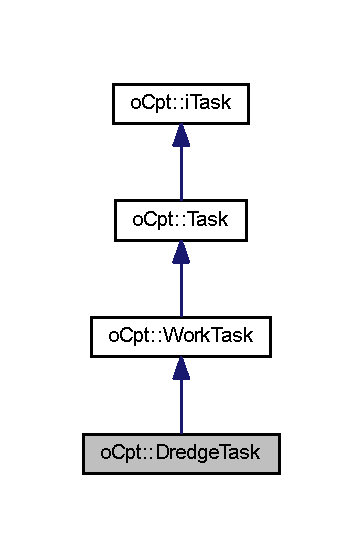
\includegraphics[width=175pt]{classo_cpt_1_1_dredge_task__inherit__graph}
\end{center}
\end{figure}


Collaboration diagram for o\+Cpt\+:\+:Dredge\+Task\+:\nopagebreak
\begin{figure}[H]
\begin{center}
\leavevmode
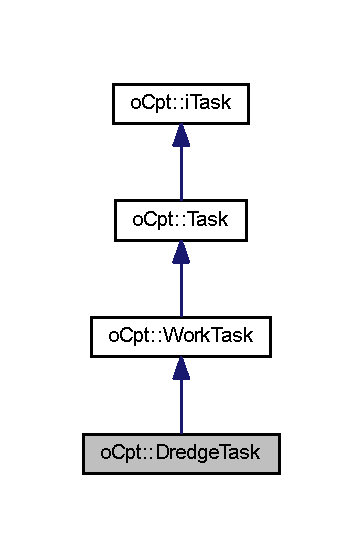
\includegraphics[width=175pt]{classo_cpt_1_1_dredge_task__coll__graph}
\end{center}
\end{figure}
\subsection*{Public Member Functions}
\begin{DoxyCompactItemize}
\item 
\hyperlink{classo_cpt_1_1_dredge_task_a959ef09f846314a23a9ad31be807f2d1}{Dredge\+Task} (\hyperlink{classo_cpt_1_1i_vessel_a43711a596f3bdfd0ca732ed3901edc97}{Vessel\+::ptr} vessel, bool concurrent=true)
\item 
virtual \hyperlink{classo_cpt_1_1_dredge_task_aa326cf6ddbb6e3019fb86f8d714bf323}{$\sim$\+Dredge\+Task} ()
\end{DoxyCompactItemize}
\subsection*{Additional Inherited Members}


\subsection{Detailed Description}
An Object representing a dredging task. 

All these types tasks make use of an actuator and sensors to perform dredging tasks 

Definition at line 287 of file Task.\+h.



\subsection{Constructor \& Destructor Documentation}
\hypertarget{classo_cpt_1_1_dredge_task_a959ef09f846314a23a9ad31be807f2d1}{}\label{classo_cpt_1_1_dredge_task_a959ef09f846314a23a9ad31be807f2d1} 
\index{o\+Cpt\+::\+Dredge\+Task@{o\+Cpt\+::\+Dredge\+Task}!Dredge\+Task@{Dredge\+Task}}
\index{Dredge\+Task@{Dredge\+Task}!o\+Cpt\+::\+Dredge\+Task@{o\+Cpt\+::\+Dredge\+Task}}
\subsubsection{\texorpdfstring{Dredge\+Task()}{DredgeTask()}}
{\footnotesize\ttfamily o\+Cpt\+::\+Dredge\+Task\+::\+Dredge\+Task (\begin{DoxyParamCaption}\item[{\hyperlink{classo_cpt_1_1i_vessel_a43711a596f3bdfd0ca732ed3901edc97}{Vessel\+::ptr}}]{vessel,  }\item[{bool}]{concurrent = {\ttfamily true} }\end{DoxyParamCaption})}

Constructor of the interface \begin{DoxyReturn}{Returns}

\end{DoxyReturn}


Definition at line 69 of file Task.\+cpp.

\hypertarget{classo_cpt_1_1_dredge_task_aa326cf6ddbb6e3019fb86f8d714bf323}{}\label{classo_cpt_1_1_dredge_task_aa326cf6ddbb6e3019fb86f8d714bf323} 
\index{o\+Cpt\+::\+Dredge\+Task@{o\+Cpt\+::\+Dredge\+Task}!````~Dredge\+Task@{$\sim$\+Dredge\+Task}}
\index{````~Dredge\+Task@{$\sim$\+Dredge\+Task}!o\+Cpt\+::\+Dredge\+Task@{o\+Cpt\+::\+Dredge\+Task}}
\subsubsection{\texorpdfstring{$\sim$\+Dredge\+Task()}{~DredgeTask()}}
{\footnotesize\ttfamily o\+Cpt\+::\+Dredge\+Task\+::$\sim$\+Dredge\+Task (\begin{DoxyParamCaption}{ }\end{DoxyParamCaption})\hspace{0.3cm}{\ttfamily [virtual]}}

The deconstructor 

Definition at line 71 of file Task.\+cpp.



The documentation for this class was generated from the following files\+:\begin{DoxyCompactItemize}
\item 
include/\+Core/\hyperlink{_task_8h}{Task.\+h}\item 
src/\+Core/\hyperlink{_task_8cpp}{Task.\+cpp}\end{DoxyCompactItemize}

\hypertarget{classo_cpt_1_1_follow_task}{}\section{o\+Cpt\+:\+:Follow\+Task Class Reference}
\label{classo_cpt_1_1_follow_task}\index{o\+Cpt\+::\+Follow\+Task@{o\+Cpt\+::\+Follow\+Task}}


An object representing a follow the target task.  




{\ttfamily \#include $<$Task.\+h$>$}

Inheritance diagram for o\+Cpt\+:\+:Follow\+Task\+:\begin{figure}[H]
\begin{center}
\leavevmode
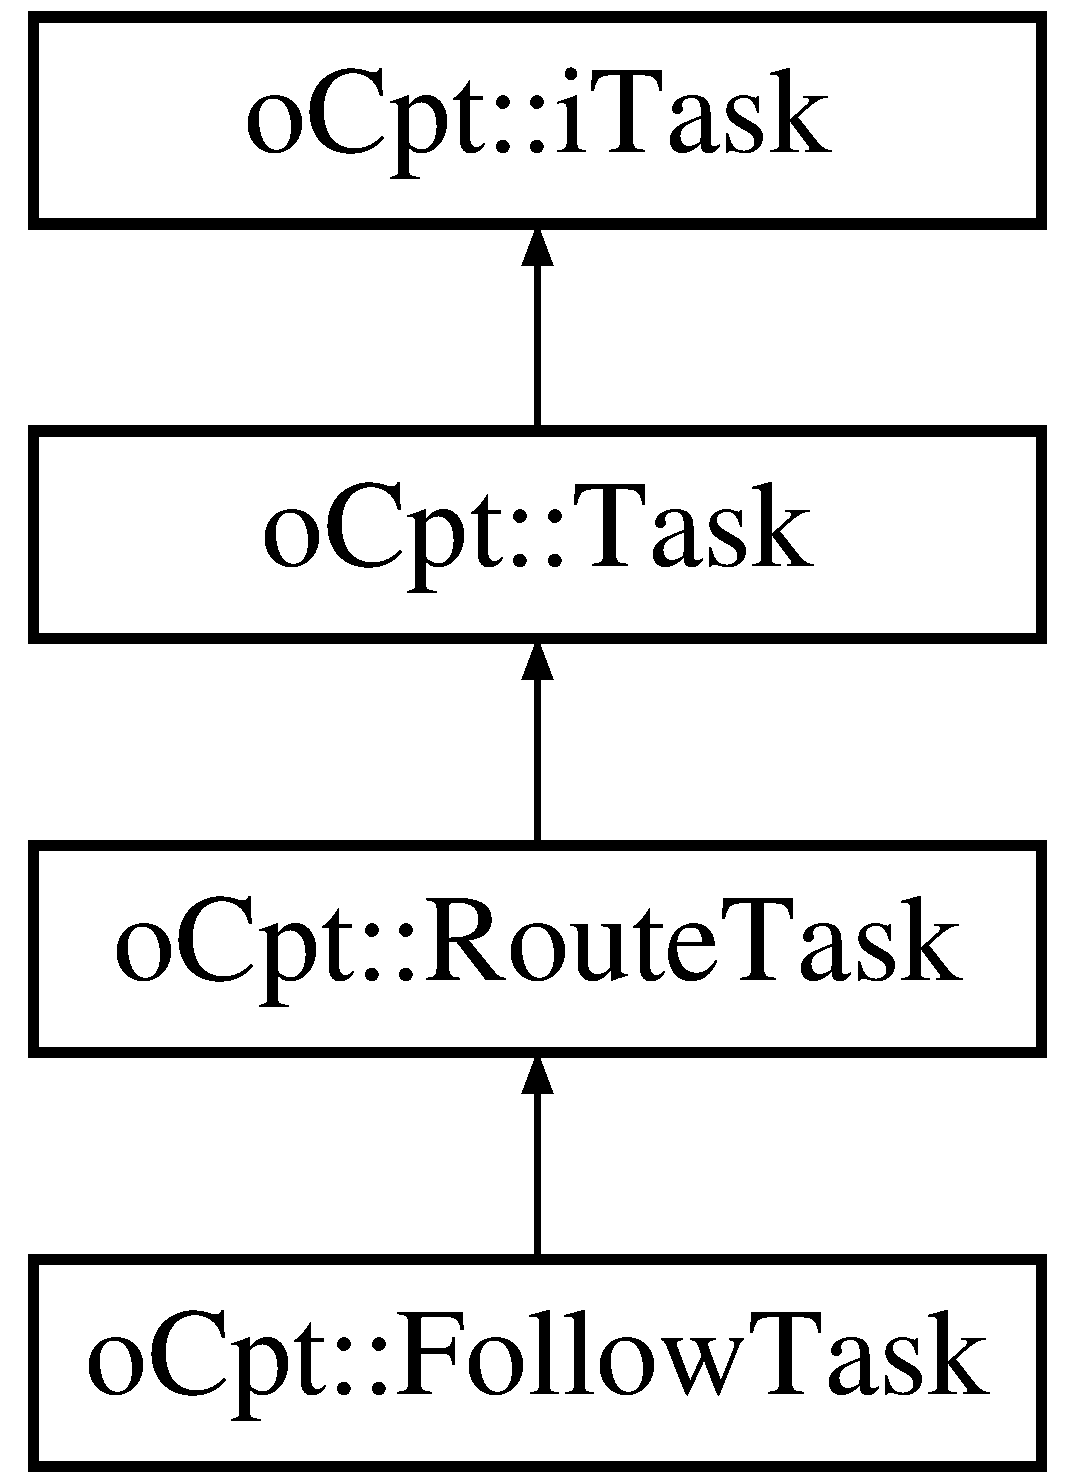
\includegraphics[height=4.000000cm]{classo_cpt_1_1_follow_task}
\end{center}
\end{figure}
\subsection*{Public Member Functions}
\begin{DoxyCompactItemize}
\item 
\hyperlink{classo_cpt_1_1_follow_task_a6e7f2d2b4037a331da8d0a994e79090c}{Follow\+Task} ()
\item 
virtual \hyperlink{classo_cpt_1_1_follow_task_ab93d2570c1e65704f6742aa5f3f6a440}{$\sim$\+Follow\+Task} ()
\end{DoxyCompactItemize}
\subsection*{Additional Inherited Members}


\subsection{Detailed Description}
An object representing a follow the target task. 

All these types of tasks need to follow a (moving) target 

\subsection{Constructor \& Destructor Documentation}
\index{o\+Cpt\+::\+Follow\+Task@{o\+Cpt\+::\+Follow\+Task}!Follow\+Task@{Follow\+Task}}
\index{Follow\+Task@{Follow\+Task}!o\+Cpt\+::\+Follow\+Task@{o\+Cpt\+::\+Follow\+Task}}
\subsubsection[{\texorpdfstring{Follow\+Task()}{FollowTask()}}]{\setlength{\rightskip}{0pt plus 5cm}o\+Cpt\+::\+Follow\+Task\+::\+Follow\+Task (
\begin{DoxyParamCaption}
{}
\end{DoxyParamCaption}
)}\hypertarget{classo_cpt_1_1_follow_task_a6e7f2d2b4037a331da8d0a994e79090c}{}\label{classo_cpt_1_1_follow_task_a6e7f2d2b4037a331da8d0a994e79090c}
Constructor of the interface \begin{DoxyReturn}{Returns}

\end{DoxyReturn}
\index{o\+Cpt\+::\+Follow\+Task@{o\+Cpt\+::\+Follow\+Task}!````~Follow\+Task@{$\sim$\+Follow\+Task}}
\index{````~Follow\+Task@{$\sim$\+Follow\+Task}!o\+Cpt\+::\+Follow\+Task@{o\+Cpt\+::\+Follow\+Task}}
\subsubsection[{\texorpdfstring{$\sim$\+Follow\+Task()}{~FollowTask()}}]{\setlength{\rightskip}{0pt plus 5cm}o\+Cpt\+::\+Follow\+Task\+::$\sim$\+Follow\+Task (
\begin{DoxyParamCaption}
{}
\end{DoxyParamCaption}
)\hspace{0.3cm}{\ttfamily [virtual]}}\hypertarget{classo_cpt_1_1_follow_task_ab93d2570c1e65704f6742aa5f3f6a440}{}\label{classo_cpt_1_1_follow_task_ab93d2570c1e65704f6742aa5f3f6a440}
The deconstructor 

The documentation for this class was generated from the following files\+:\begin{DoxyCompactItemize}
\item 
include/\hyperlink{_task_8h}{Task.\+h}\item 
src/\hyperlink{_task_8cpp}{Task.\+cpp}\end{DoxyCompactItemize}

\hypertarget{classo_cpt_1_1i_task}{}\section{o\+Cpt\+:\+:i\+Task Class Reference}
\label{classo_cpt_1_1i_task}\index{o\+Cpt\+::i\+Task@{o\+Cpt\+::i\+Task}}


\hyperlink{classo_cpt_1_1_task}{Task} interface, all tasks need to adhere to this structure.  




{\ttfamily \#include $<$Task.\+h$>$}



Inheritance diagram for o\+Cpt\+:\+:i\+Task\+:\nopagebreak
\begin{figure}[H]
\begin{center}
\leavevmode
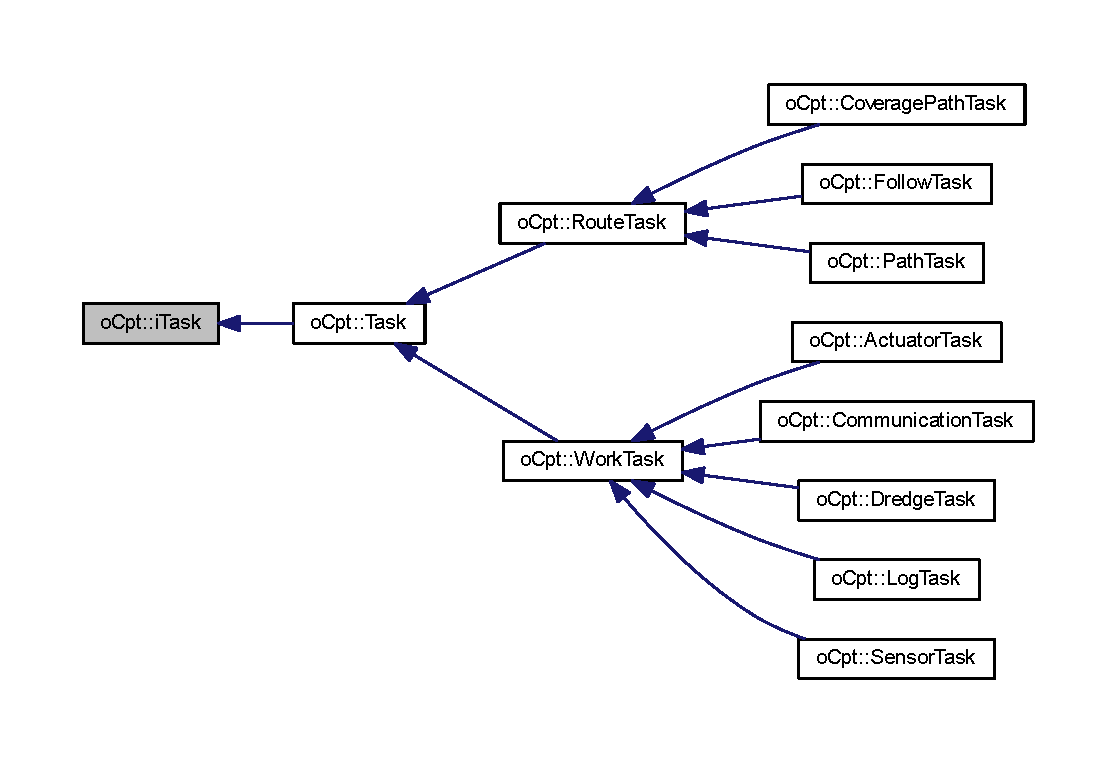
\includegraphics[width=350pt]{classo_cpt_1_1i_task__inherit__graph}
\end{center}
\end{figure}
\subsection*{Classes}
\begin{DoxyCompactItemize}
\item 
class \hyperlink{classo_cpt_1_1i_task_1_1_status}{Status}
\end{DoxyCompactItemize}
\subsection*{Public Types}
\begin{DoxyCompactItemize}
\item 
enum \hyperlink{classo_cpt_1_1i_task_a10d8726eb8957c2c305f468cf15b9f11}{Type\+Of} \{ \hyperlink{classo_cpt_1_1i_task_a10d8726eb8957c2c305f468cf15b9f11a7ca85240095e3a76c70f5535d26c4dd3}{R\+O\+U\+TE} = 1, 
\hyperlink{classo_cpt_1_1i_task_a10d8726eb8957c2c305f468cf15b9f11a1ec34e80717bb96ddd8376ff12d1b4c9}{W\+O\+RK} = 2
 \}
\item 
typedef boost\+::shared\+\_\+ptr$<$ \hyperlink{classo_cpt_1_1i_task}{i\+Task} $>$ \hyperlink{classo_cpt_1_1i_task_add2b02b5c97e63a1b7d6943ea4571543}{ptr}
\begin{DoxyCompactList}\small\item\em Boost shared\+\_\+ptr to a task. \end{DoxyCompactList}\item 
typedef std\+::list$<$ \hyperlink{classo_cpt_1_1i_task_add2b02b5c97e63a1b7d6943ea4571543}{i\+Task\+::ptr} $>$ \hyperlink{classo_cpt_1_1i_task_a8f949d091241347ea0cdfb8625b4dbca}{taskqueue}
\begin{DoxyCompactList}\small\item\em A list of shared pointer tasks. \end{DoxyCompactList}\end{DoxyCompactItemize}
\subsection*{Public Member Functions}
\begin{DoxyCompactItemize}
\item 
\hyperlink{classo_cpt_1_1i_task_a5b5affdc2f5213d8c5f11e8cd1cda517}{i\+Task} (\hyperlink{classo_cpt_1_1i_vessel_a43711a596f3bdfd0ca732ed3901edc97}{i\+Vessel\+::ptr} vessel, bool concurrent=false)
\item 
virtual \hyperlink{classo_cpt_1_1i_task_aa2c1053421fff92430b5912e0d3c7fc7}{$\sim$i\+Task} ()
\item 
virtual void \hyperlink{classo_cpt_1_1i_task_aedd48e3c4df48aaae0738ce3863e222f}{start} ()=0
\item 
virtual \hyperlink{classo_cpt_1_1i_task_1_1_status_aaf766c58d038e2defc3de2dddb92d1eb}{i\+Task\+::\+Status\+::ptr} \hyperlink{classo_cpt_1_1i_task_a8d6126b2e337a0ab39fdef1d8d7b73b9}{status} ()=0
\item 
virtual void \hyperlink{classo_cpt_1_1i_task_aedb88813b16914598dee9561813e56e8}{stop} ()=0
\end{DoxyCompactItemize}
\subsection*{Public Attributes}
\begin{DoxyCompactItemize}
\item 
\hyperlink{classo_cpt_1_1i_task_a8f949d091241347ea0cdfb8625b4dbca}{taskqueue} \hyperlink{classo_cpt_1_1i_task_a41287056bebbed04966072dfd1a9f80f}{Work}
\end{DoxyCompactItemize}
\subsection*{Protected Attributes}
\begin{DoxyCompactItemize}
\item 
bool \hyperlink{classo_cpt_1_1i_task_a1b6eaff4578d2ff18e70b07d00d7bb45}{\+\_\+concurrent} = false
\begin{DoxyCompactList}\small\item\em Allowed to run as a seperate thread. \end{DoxyCompactList}\item 
\hyperlink{classo_cpt_1_1i_vessel_a43711a596f3bdfd0ca732ed3901edc97}{Vessel\+::ptr} \hyperlink{classo_cpt_1_1i_task_ac6cc57220c87f87cdd4d1749119ae0cb}{\+\_\+vessel} = nullptr
\begin{DoxyCompactList}\small\item\em Pointer to the world. \end{DoxyCompactList}\end{DoxyCompactItemize}


\subsection{Detailed Description}
\hyperlink{classo_cpt_1_1_task}{Task} interface, all tasks need to adhere to this structure. 

This interface make sure that all task adheres to the same runtime rules and enable run-\/time polymorphism 

Definition at line 20 of file Task.\+h.



\subsection{Member Typedef Documentation}
\hypertarget{classo_cpt_1_1i_task_add2b02b5c97e63a1b7d6943ea4571543}{}\label{classo_cpt_1_1i_task_add2b02b5c97e63a1b7d6943ea4571543} 
\index{o\+Cpt\+::i\+Task@{o\+Cpt\+::i\+Task}!ptr@{ptr}}
\index{ptr@{ptr}!o\+Cpt\+::i\+Task@{o\+Cpt\+::i\+Task}}
\subsubsection{\texorpdfstring{ptr}{ptr}}
{\footnotesize\ttfamily typedef boost\+::shared\+\_\+ptr$<$\hyperlink{classo_cpt_1_1i_task}{i\+Task}$>$ \hyperlink{classo_cpt_1_1i_task_add2b02b5c97e63a1b7d6943ea4571543}{o\+Cpt\+::i\+Task\+::ptr}}



Boost shared\+\_\+ptr to a task. 



Definition at line 22 of file Task.\+h.

\hypertarget{classo_cpt_1_1i_task_a8f949d091241347ea0cdfb8625b4dbca}{}\label{classo_cpt_1_1i_task_a8f949d091241347ea0cdfb8625b4dbca} 
\index{o\+Cpt\+::i\+Task@{o\+Cpt\+::i\+Task}!taskqueue@{taskqueue}}
\index{taskqueue@{taskqueue}!o\+Cpt\+::i\+Task@{o\+Cpt\+::i\+Task}}
\subsubsection{\texorpdfstring{taskqueue}{taskqueue}}
{\footnotesize\ttfamily typedef std\+::list$<$\hyperlink{classo_cpt_1_1i_task_add2b02b5c97e63a1b7d6943ea4571543}{i\+Task\+::ptr}$>$ \hyperlink{classo_cpt_1_1i_task_a8f949d091241347ea0cdfb8625b4dbca}{o\+Cpt\+::i\+Task\+::taskqueue}}



A list of shared pointer tasks. 



Definition at line 23 of file Task.\+h.



\subsection{Member Enumeration Documentation}
\hypertarget{classo_cpt_1_1i_task_a10d8726eb8957c2c305f468cf15b9f11}{}\label{classo_cpt_1_1i_task_a10d8726eb8957c2c305f468cf15b9f11} 
\index{o\+Cpt\+::i\+Task@{o\+Cpt\+::i\+Task}!Type\+Of@{Type\+Of}}
\index{Type\+Of@{Type\+Of}!o\+Cpt\+::i\+Task@{o\+Cpt\+::i\+Task}}
\subsubsection{\texorpdfstring{Type\+Of}{TypeOf}}
{\footnotesize\ttfamily enum \hyperlink{classo_cpt_1_1i_task_a10d8726eb8957c2c305f468cf15b9f11}{o\+Cpt\+::i\+Task\+::\+Type\+Of}}

Enumeration indicating which type of task the object is \begin{DoxyEnumFields}{Enumerator}
\raisebox{\heightof{T}}[0pt][0pt]{\index{R\+O\+U\+TE@{R\+O\+U\+TE}!o\+Cpt\+::i\+Task@{o\+Cpt\+::i\+Task}}\index{o\+Cpt\+::i\+Task@{o\+Cpt\+::i\+Task}!R\+O\+U\+TE@{R\+O\+U\+TE}}}\hypertarget{classo_cpt_1_1i_task_a10d8726eb8957c2c305f468cf15b9f11a7ca85240095e3a76c70f5535d26c4dd3}{}\label{classo_cpt_1_1i_task_a10d8726eb8957c2c305f468cf15b9f11a7ca85240095e3a76c70f5535d26c4dd3} 
R\+O\+U\+TE&\\
\hline

\raisebox{\heightof{T}}[0pt][0pt]{\index{W\+O\+RK@{W\+O\+RK}!o\+Cpt\+::i\+Task@{o\+Cpt\+::i\+Task}}\index{o\+Cpt\+::i\+Task@{o\+Cpt\+::i\+Task}!W\+O\+RK@{W\+O\+RK}}}\hypertarget{classo_cpt_1_1i_task_a10d8726eb8957c2c305f468cf15b9f11a1ec34e80717bb96ddd8376ff12d1b4c9}{}\label{classo_cpt_1_1i_task_a10d8726eb8957c2c305f468cf15b9f11a1ec34e80717bb96ddd8376ff12d1b4c9} 
W\+O\+RK&\\
\hline

\end{DoxyEnumFields}


Definition at line 72 of file Task.\+h.



\subsection{Constructor \& Destructor Documentation}
\hypertarget{classo_cpt_1_1i_task_a5b5affdc2f5213d8c5f11e8cd1cda517}{}\label{classo_cpt_1_1i_task_a5b5affdc2f5213d8c5f11e8cd1cda517} 
\index{o\+Cpt\+::i\+Task@{o\+Cpt\+::i\+Task}!i\+Task@{i\+Task}}
\index{i\+Task@{i\+Task}!o\+Cpt\+::i\+Task@{o\+Cpt\+::i\+Task}}
\subsubsection{\texorpdfstring{i\+Task()}{iTask()}}
{\footnotesize\ttfamily o\+Cpt\+::i\+Task\+::i\+Task (\begin{DoxyParamCaption}\item[{\hyperlink{classo_cpt_1_1i_vessel_a43711a596f3bdfd0ca732ed3901edc97}{i\+Vessel\+::ptr}}]{vessel,  }\item[{bool}]{concurrent = {\ttfamily false} }\end{DoxyParamCaption})}

Constructor of the interface \begin{DoxyReturn}{Returns}

\end{DoxyReturn}


Definition at line 8 of file Task.\+cpp.



References \+\_\+concurrent, and \+\_\+vessel.

\hypertarget{classo_cpt_1_1i_task_aa2c1053421fff92430b5912e0d3c7fc7}{}\label{classo_cpt_1_1i_task_aa2c1053421fff92430b5912e0d3c7fc7} 
\index{o\+Cpt\+::i\+Task@{o\+Cpt\+::i\+Task}!````~i\+Task@{$\sim$i\+Task}}
\index{````~i\+Task@{$\sim$i\+Task}!o\+Cpt\+::i\+Task@{o\+Cpt\+::i\+Task}}
\subsubsection{\texorpdfstring{$\sim$i\+Task()}{~iTask()}}
{\footnotesize\ttfamily o\+Cpt\+::i\+Task\+::$\sim$i\+Task (\begin{DoxyParamCaption}{ }\end{DoxyParamCaption})\hspace{0.3cm}{\ttfamily [virtual]}}

Deconstructor of the interface 

Definition at line 13 of file Task.\+cpp.



\subsection{Member Function Documentation}
\hypertarget{classo_cpt_1_1i_task_aedd48e3c4df48aaae0738ce3863e222f}{}\label{classo_cpt_1_1i_task_aedd48e3c4df48aaae0738ce3863e222f} 
\index{o\+Cpt\+::i\+Task@{o\+Cpt\+::i\+Task}!start@{start}}
\index{start@{start}!o\+Cpt\+::i\+Task@{o\+Cpt\+::i\+Task}}
\subsubsection{\texorpdfstring{start()}{start()}}
{\footnotesize\ttfamily virtual void o\+Cpt\+::i\+Task\+::start (\begin{DoxyParamCaption}{ }\end{DoxyParamCaption})\hspace{0.3cm}{\ttfamily [pure virtual]}}

The start command for a task 

Implemented in \hyperlink{classo_cpt_1_1_task_a8acd8d2125df0aef37eb1ebf0e3e49c8}{o\+Cpt\+::\+Task}.

\hypertarget{classo_cpt_1_1i_task_a8d6126b2e337a0ab39fdef1d8d7b73b9}{}\label{classo_cpt_1_1i_task_a8d6126b2e337a0ab39fdef1d8d7b73b9} 
\index{o\+Cpt\+::i\+Task@{o\+Cpt\+::i\+Task}!status@{status}}
\index{status@{status}!o\+Cpt\+::i\+Task@{o\+Cpt\+::i\+Task}}
\subsubsection{\texorpdfstring{status()}{status()}}
{\footnotesize\ttfamily virtual \hyperlink{classo_cpt_1_1i_task_1_1_status_aaf766c58d038e2defc3de2dddb92d1eb}{i\+Task\+::\+Status\+::ptr} o\+Cpt\+::i\+Task\+::status (\begin{DoxyParamCaption}{ }\end{DoxyParamCaption})\hspace{0.3cm}{\ttfamily [pure virtual]}}

Retrieves the \hyperlink{classo_cpt_1_1i_task_1_1_status}{Status} of a task \begin{DoxyReturn}{Returns}
Boost shared\+\_\+ptr of the task status 
\end{DoxyReturn}


Implemented in \hyperlink{classo_cpt_1_1_task_a724445e158919a4b5644d8eef9f7c754}{o\+Cpt\+::\+Task}.

\hypertarget{classo_cpt_1_1i_task_aedb88813b16914598dee9561813e56e8}{}\label{classo_cpt_1_1i_task_aedb88813b16914598dee9561813e56e8} 
\index{o\+Cpt\+::i\+Task@{o\+Cpt\+::i\+Task}!stop@{stop}}
\index{stop@{stop}!o\+Cpt\+::i\+Task@{o\+Cpt\+::i\+Task}}
\subsubsection{\texorpdfstring{stop()}{stop()}}
{\footnotesize\ttfamily virtual void o\+Cpt\+::i\+Task\+::stop (\begin{DoxyParamCaption}{ }\end{DoxyParamCaption})\hspace{0.3cm}{\ttfamily [pure virtual]}}

The stop command for a task 

Implemented in \hyperlink{classo_cpt_1_1_task_a62b4f1bbc1cf24434d2a2130162507f7}{o\+Cpt\+::\+Task}.



\subsection{Member Data Documentation}
\hypertarget{classo_cpt_1_1i_task_a1b6eaff4578d2ff18e70b07d00d7bb45}{}\label{classo_cpt_1_1i_task_a1b6eaff4578d2ff18e70b07d00d7bb45} 
\index{o\+Cpt\+::i\+Task@{o\+Cpt\+::i\+Task}!\+\_\+concurrent@{\+\_\+concurrent}}
\index{\+\_\+concurrent@{\+\_\+concurrent}!o\+Cpt\+::i\+Task@{o\+Cpt\+::i\+Task}}
\subsubsection{\texorpdfstring{\+\_\+concurrent}{\_concurrent}}
{\footnotesize\ttfamily bool o\+Cpt\+::i\+Task\+::\+\_\+concurrent = false\hspace{0.3cm}{\ttfamily [protected]}}



Allowed to run as a seperate thread. 



Definition at line 104 of file Task.\+h.



Referenced by i\+Task().

\hypertarget{classo_cpt_1_1i_task_ac6cc57220c87f87cdd4d1749119ae0cb}{}\label{classo_cpt_1_1i_task_ac6cc57220c87f87cdd4d1749119ae0cb} 
\index{o\+Cpt\+::i\+Task@{o\+Cpt\+::i\+Task}!\+\_\+vessel@{\+\_\+vessel}}
\index{\+\_\+vessel@{\+\_\+vessel}!o\+Cpt\+::i\+Task@{o\+Cpt\+::i\+Task}}
\subsubsection{\texorpdfstring{\+\_\+vessel}{\_vessel}}
{\footnotesize\ttfamily \hyperlink{classo_cpt_1_1i_vessel_a43711a596f3bdfd0ca732ed3901edc97}{Vessel\+::ptr} o\+Cpt\+::i\+Task\+::\+\_\+vessel = nullptr\hspace{0.3cm}{\ttfamily [protected]}}



Pointer to the world. 



Definition at line 105 of file Task.\+h.



Referenced by i\+Task().

\hypertarget{classo_cpt_1_1i_task_a41287056bebbed04966072dfd1a9f80f}{}\label{classo_cpt_1_1i_task_a41287056bebbed04966072dfd1a9f80f} 
\index{o\+Cpt\+::i\+Task@{o\+Cpt\+::i\+Task}!Work@{Work}}
\index{Work@{Work}!o\+Cpt\+::i\+Task@{o\+Cpt\+::i\+Task}}
\subsubsection{\texorpdfstring{Work}{Work}}
{\footnotesize\ttfamily \hyperlink{classo_cpt_1_1i_task_a8f949d091241347ea0cdfb8625b4dbca}{taskqueue} o\+Cpt\+::i\+Task\+::\+Work}



Definition at line 25 of file Task.\+h.



Referenced by o\+Cpt\+::\+Task\+::start().



The documentation for this class was generated from the following files\+:\begin{DoxyCompactItemize}
\item 
/projects/mti/oh\+Captain/oh\+Captain/include/\+Core/\hyperlink{_task_8h}{Task.\+h}\item 
/projects/mti/oh\+Captain/oh\+Captain/src/\+Core/\hyperlink{_task_8cpp}{Task.\+cpp}\end{DoxyCompactItemize}

\hypertarget{classo_cpt_1_1_log_task}{}\section{o\+Cpt\+:\+:Log\+Task Class Reference}
\label{classo_cpt_1_1_log_task}\index{o\+Cpt\+::\+Log\+Task@{o\+Cpt\+::\+Log\+Task}}


An Object representing a data logging task.  




{\ttfamily \#include $<$Task.\+h$>$}

Inheritance diagram for o\+Cpt\+:\+:Log\+Task\+:\begin{figure}[H]
\begin{center}
\leavevmode
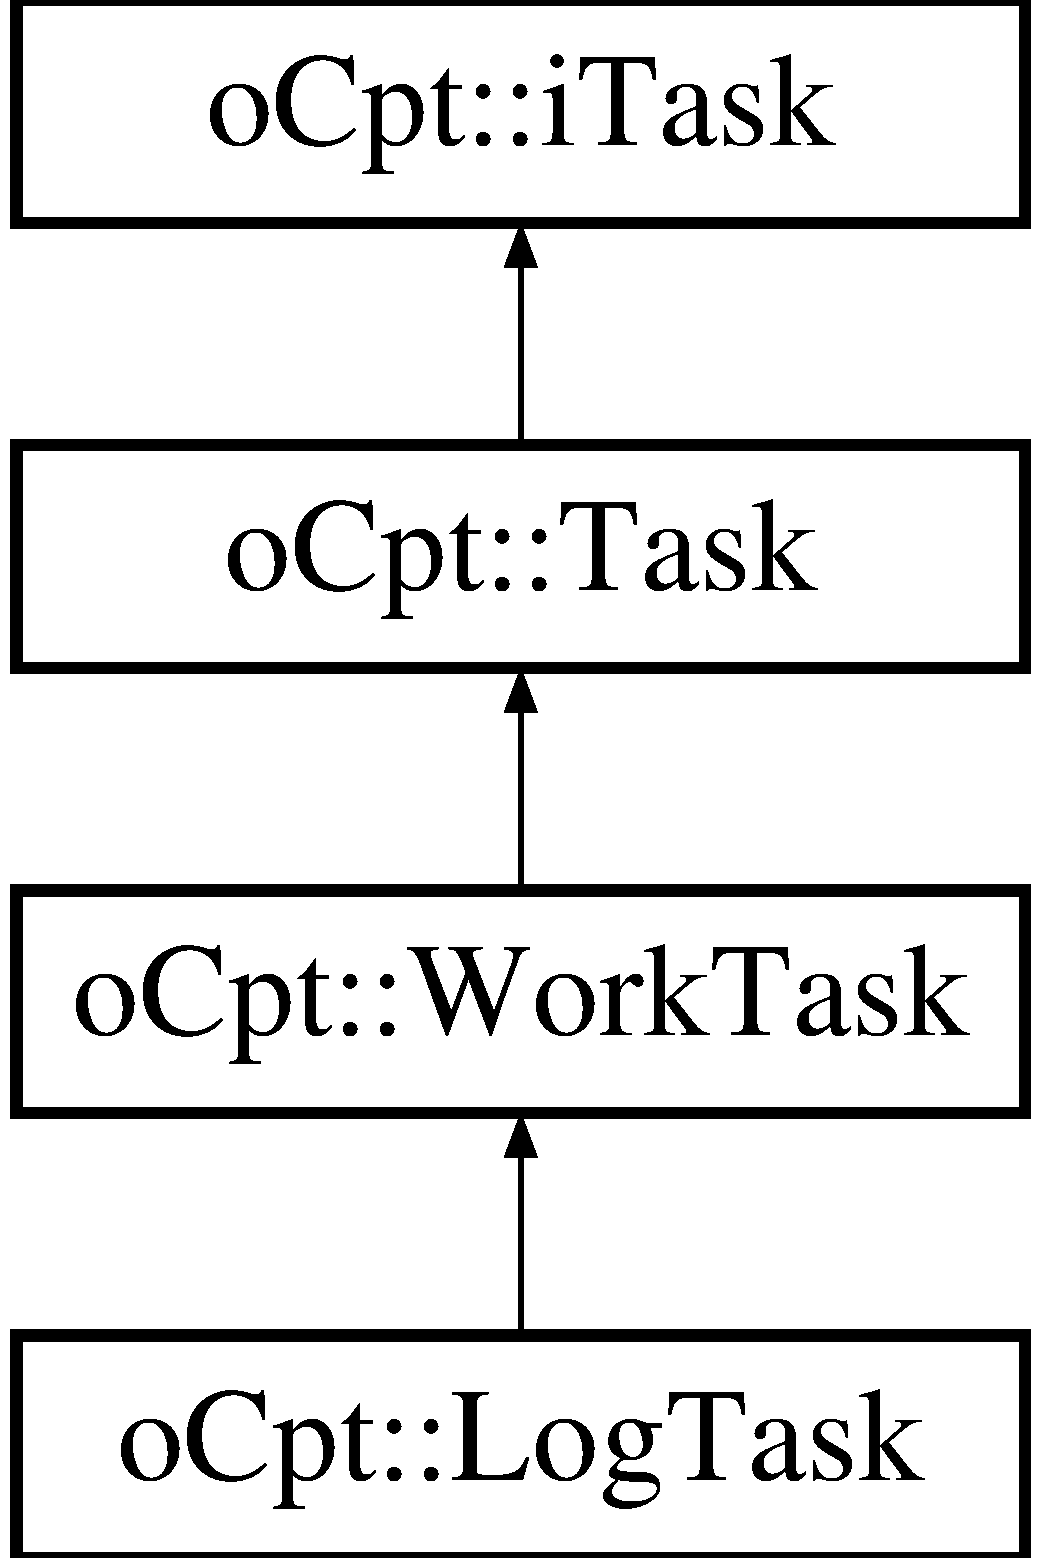
\includegraphics[height=4.000000cm]{classo_cpt_1_1_log_task}
\end{center}
\end{figure}
\subsection*{Public Member Functions}
\begin{DoxyCompactItemize}
\item 
\hyperlink{classo_cpt_1_1_log_task_aac2dc42f834a76d4eb374ed568d92db9}{Log\+Task} ()
\item 
virtual \hyperlink{classo_cpt_1_1_log_task_a0f80363644cbe0a9c17e78198d466788}{$\sim$\+Log\+Task} ()
\end{DoxyCompactItemize}
\subsection*{Additional Inherited Members}


\subsection{Detailed Description}
An Object representing a data logging task. 

All these types of tasks make use of a sensor to record and log 

\subsection{Constructor \& Destructor Documentation}
\index{o\+Cpt\+::\+Log\+Task@{o\+Cpt\+::\+Log\+Task}!Log\+Task@{Log\+Task}}
\index{Log\+Task@{Log\+Task}!o\+Cpt\+::\+Log\+Task@{o\+Cpt\+::\+Log\+Task}}
\subsubsection[{\texorpdfstring{Log\+Task()}{LogTask()}}]{\setlength{\rightskip}{0pt plus 5cm}o\+Cpt\+::\+Log\+Task\+::\+Log\+Task (
\begin{DoxyParamCaption}
{}
\end{DoxyParamCaption}
)}\hypertarget{classo_cpt_1_1_log_task_aac2dc42f834a76d4eb374ed568d92db9}{}\label{classo_cpt_1_1_log_task_aac2dc42f834a76d4eb374ed568d92db9}
Constructor of the interface \begin{DoxyReturn}{Returns}

\end{DoxyReturn}
\index{o\+Cpt\+::\+Log\+Task@{o\+Cpt\+::\+Log\+Task}!````~Log\+Task@{$\sim$\+Log\+Task}}
\index{````~Log\+Task@{$\sim$\+Log\+Task}!o\+Cpt\+::\+Log\+Task@{o\+Cpt\+::\+Log\+Task}}
\subsubsection[{\texorpdfstring{$\sim$\+Log\+Task()}{~LogTask()}}]{\setlength{\rightskip}{0pt plus 5cm}o\+Cpt\+::\+Log\+Task\+::$\sim$\+Log\+Task (
\begin{DoxyParamCaption}
{}
\end{DoxyParamCaption}
)\hspace{0.3cm}{\ttfamily [virtual]}}\hypertarget{classo_cpt_1_1_log_task_a0f80363644cbe0a9c17e78198d466788}{}\label{classo_cpt_1_1_log_task_a0f80363644cbe0a9c17e78198d466788}
The deconstructor 

The documentation for this class was generated from the following files\+:\begin{DoxyCompactItemize}
\item 
include/\hyperlink{_task_8h}{Task.\+h}\item 
src/\hyperlink{_task_8cpp}{Task.\+cpp}\end{DoxyCompactItemize}

\hypertarget{classo_cpt_1_1_path_task}{}\section{o\+Cpt\+:\+:Path\+Task Class Reference}
\label{classo_cpt_1_1_path_task}\index{o\+Cpt\+::\+Path\+Task@{o\+Cpt\+::\+Path\+Task}}


An object representing a normal A to B type of path planning.  




{\ttfamily \#include $<$Task.\+h$>$}



Inheritance diagram for o\+Cpt\+:\+:Path\+Task\+:\nopagebreak
\begin{figure}[H]
\begin{center}
\leavevmode
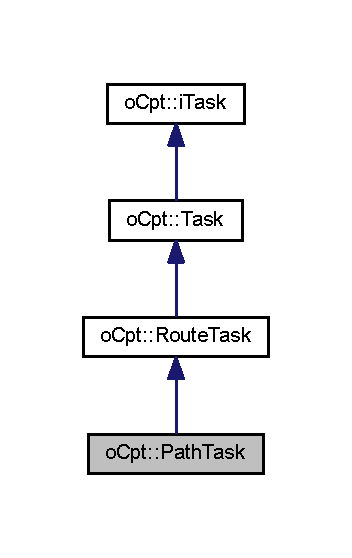
\includegraphics[width=169pt]{classo_cpt_1_1_path_task__inherit__graph}
\end{center}
\end{figure}


Collaboration diagram for o\+Cpt\+:\+:Path\+Task\+:\nopagebreak
\begin{figure}[H]
\begin{center}
\leavevmode
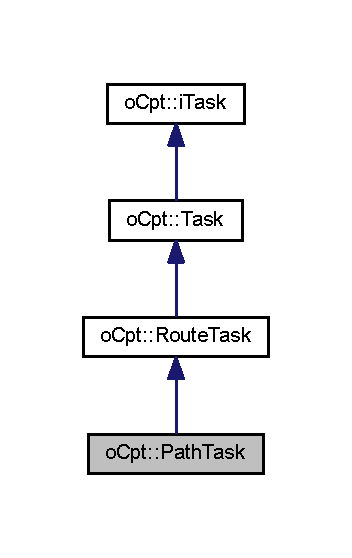
\includegraphics[width=169pt]{classo_cpt_1_1_path_task__coll__graph}
\end{center}
\end{figure}
\subsection*{Public Member Functions}
\begin{DoxyCompactItemize}
\item 
\hyperlink{classo_cpt_1_1_path_task_a3ea7676103564aaaca3b933c95c3f6c6}{Path\+Task} (\hyperlink{classo_cpt_1_1i_vessel_a43711a596f3bdfd0ca732ed3901edc97}{Vessel\+::ptr} vessel, bool concurrent=false)
\item 
virtual \hyperlink{classo_cpt_1_1_path_task_a957810982a8f94b7c0b942e348e86467}{$\sim$\+Path\+Task} ()
\end{DoxyCompactItemize}
\subsection*{Additional Inherited Members}


\subsection{Detailed Description}
An object representing a normal A to B type of path planning. 

All these types of tasks need to plann an optimum route between A and B, either in time, energy consumption or 

Definition at line 244 of file Task.\+h.



\subsection{Constructor \& Destructor Documentation}
\hypertarget{classo_cpt_1_1_path_task_a3ea7676103564aaaca3b933c95c3f6c6}{}\label{classo_cpt_1_1_path_task_a3ea7676103564aaaca3b933c95c3f6c6} 
\index{o\+Cpt\+::\+Path\+Task@{o\+Cpt\+::\+Path\+Task}!Path\+Task@{Path\+Task}}
\index{Path\+Task@{Path\+Task}!o\+Cpt\+::\+Path\+Task@{o\+Cpt\+::\+Path\+Task}}
\subsubsection{\texorpdfstring{Path\+Task()}{PathTask()}}
{\footnotesize\ttfamily o\+Cpt\+::\+Path\+Task\+::\+Path\+Task (\begin{DoxyParamCaption}\item[{\hyperlink{classo_cpt_1_1i_vessel_a43711a596f3bdfd0ca732ed3901edc97}{Vessel\+::ptr}}]{vessel,  }\item[{bool}]{concurrent = {\ttfamily false} }\end{DoxyParamCaption})}

Constructor of the interface \begin{DoxyReturn}{Returns}

\end{DoxyReturn}


Definition at line 61 of file Task.\+cpp.

\hypertarget{classo_cpt_1_1_path_task_a957810982a8f94b7c0b942e348e86467}{}\label{classo_cpt_1_1_path_task_a957810982a8f94b7c0b942e348e86467} 
\index{o\+Cpt\+::\+Path\+Task@{o\+Cpt\+::\+Path\+Task}!````~Path\+Task@{$\sim$\+Path\+Task}}
\index{````~Path\+Task@{$\sim$\+Path\+Task}!o\+Cpt\+::\+Path\+Task@{o\+Cpt\+::\+Path\+Task}}
\subsubsection{\texorpdfstring{$\sim$\+Path\+Task()}{~PathTask()}}
{\footnotesize\ttfamily o\+Cpt\+::\+Path\+Task\+::$\sim$\+Path\+Task (\begin{DoxyParamCaption}{ }\end{DoxyParamCaption})\hspace{0.3cm}{\ttfamily [virtual]}}

The deconstructor 

Definition at line 63 of file Task.\+cpp.



The documentation for this class was generated from the following files\+:\begin{DoxyCompactItemize}
\item 
include/\+Core/\hyperlink{_task_8h}{Task.\+h}\item 
src/\+Core/\hyperlink{_task_8cpp}{Task.\+cpp}\end{DoxyCompactItemize}

\hypertarget{classo_cpt_1_1_route_task}{}\section{o\+Cpt\+:\+:Route\+Task Class Reference}
\label{classo_cpt_1_1_route_task}\index{o\+Cpt\+::\+Route\+Task@{o\+Cpt\+::\+Route\+Task}}


{\ttfamily \#include $<$Task.\+h$>$}

Inheritance diagram for o\+Cpt\+:\+:Route\+Task\+:\begin{figure}[H]
\begin{center}
\leavevmode
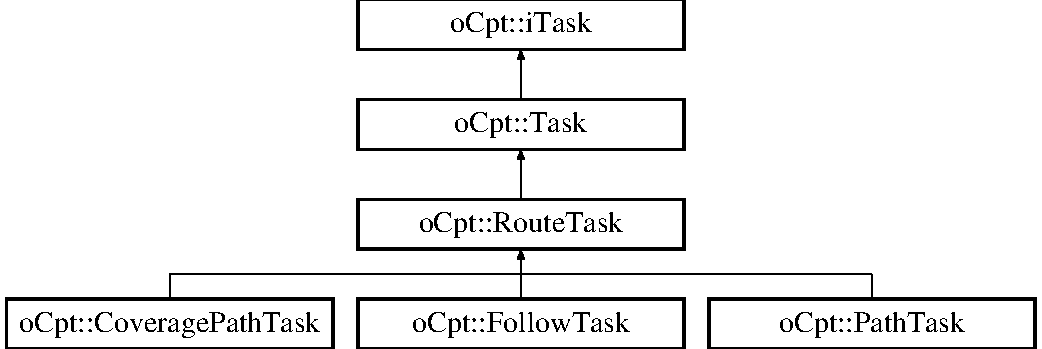
\includegraphics[height=4.000000cm]{classo_cpt_1_1_route_task}
\end{center}
\end{figure}
\subsection*{Public Member Functions}
\begin{DoxyCompactItemize}
\item 
\hyperlink{classo_cpt_1_1_route_task_a55e83da33e340ad00976eabab10ebe0c}{Route\+Task} ()
\item 
virtual \hyperlink{classo_cpt_1_1_route_task_a036b646437996f15a9e74bc12c14aa35}{$\sim$\+Route\+Task} ()
\end{DoxyCompactItemize}
\subsection*{Additional Inherited Members}


\subsection{Detailed Description}
An object repsressenting route related tasks 

\subsection{Constructor \& Destructor Documentation}
\index{o\+Cpt\+::\+Route\+Task@{o\+Cpt\+::\+Route\+Task}!Route\+Task@{Route\+Task}}
\index{Route\+Task@{Route\+Task}!o\+Cpt\+::\+Route\+Task@{o\+Cpt\+::\+Route\+Task}}
\subsubsection[{\texorpdfstring{Route\+Task()}{RouteTask()}}]{\setlength{\rightskip}{0pt plus 5cm}o\+Cpt\+::\+Route\+Task\+::\+Route\+Task (
\begin{DoxyParamCaption}
{}
\end{DoxyParamCaption}
)}\hypertarget{classo_cpt_1_1_route_task_a55e83da33e340ad00976eabab10ebe0c}{}\label{classo_cpt_1_1_route_task_a55e83da33e340ad00976eabab10ebe0c}
Constructor of the interface \begin{DoxyReturn}{Returns}

\end{DoxyReturn}
\index{o\+Cpt\+::\+Route\+Task@{o\+Cpt\+::\+Route\+Task}!````~Route\+Task@{$\sim$\+Route\+Task}}
\index{````~Route\+Task@{$\sim$\+Route\+Task}!o\+Cpt\+::\+Route\+Task@{o\+Cpt\+::\+Route\+Task}}
\subsubsection[{\texorpdfstring{$\sim$\+Route\+Task()}{~RouteTask()}}]{\setlength{\rightskip}{0pt plus 5cm}o\+Cpt\+::\+Route\+Task\+::$\sim$\+Route\+Task (
\begin{DoxyParamCaption}
{}
\end{DoxyParamCaption}
)\hspace{0.3cm}{\ttfamily [virtual]}}\hypertarget{classo_cpt_1_1_route_task_a036b646437996f15a9e74bc12c14aa35}{}\label{classo_cpt_1_1_route_task_a036b646437996f15a9e74bc12c14aa35}
The deconstructor 

The documentation for this class was generated from the following files\+:\begin{DoxyCompactItemize}
\item 
include/\hyperlink{_task_8h}{Task.\+h}\item 
src/\hyperlink{_task_8cpp}{Task.\+cpp}\end{DoxyCompactItemize}

\hypertarget{classo_cpt_1_1i_task_1_1_status}{}\section{o\+Cpt\+:\+:i\+Task\+:\+:Status Class Reference}
\label{classo_cpt_1_1i_task_1_1_status}\index{o\+Cpt\+::i\+Task\+::\+Status@{o\+Cpt\+::i\+Task\+::\+Status}}


{\ttfamily \#include $<$Task.\+h$>$}

\subsection*{Public Types}
\begin{DoxyCompactItemize}
\item 
typedef boost\+::shared\+\_\+ptr$<$ \hyperlink{classo_cpt_1_1i_task_1_1_status}{i\+Task\+::\+Status} $>$ \hyperlink{classo_cpt_1_1i_task_1_1_status_aaf766c58d038e2defc3de2dddb92d1eb}{ptr}
\begin{DoxyCompactList}\small\item\em Boost shared\+\_\+ptr to the task status. \end{DoxyCompactList}\end{DoxyCompactItemize}
\subsection*{Public Member Functions}
\begin{DoxyCompactItemize}
\item 
\hyperlink{classo_cpt_1_1i_task_1_1_status_a5fab36410db264d0b9815f34227f33d0}{Status} ()
\item 
virtual \hyperlink{classo_cpt_1_1i_task_1_1_status_a80bab1abd55406ce11f5878c2bf5f500}{$\sim$\+Status} ()
\item 
double \hyperlink{classo_cpt_1_1i_task_1_1_status_abc4f40acb0a7b5f73407cefb01187ae8}{progress} ()
\item 
bool \hyperlink{classo_cpt_1_1i_task_1_1_status_aeaab915a0c1d317727087f070d5d64a1}{running} ()
\item 
bool \hyperlink{classo_cpt_1_1i_task_1_1_status_a4140c14ea06f86f87553fa979ccd1836}{successful} ()
\end{DoxyCompactItemize}
\subsection*{Private Attributes}
\begin{DoxyCompactItemize}
\item 
double \hyperlink{classo_cpt_1_1i_task_1_1_status_acaf00b89021b6b962cc0fe8d8ea01b85}{\+\_\+progress} = 0.\+0
\item 
bool \hyperlink{classo_cpt_1_1i_task_1_1_status_ab9896a94738163478468028599a8e4f7}{\+\_\+running} = false
\item 
bool \hyperlink{classo_cpt_1_1i_task_1_1_status_acac4794c074b5483c0c05f68c3689df9}{\+\_\+successful}
\end{DoxyCompactItemize}


\subsection{Detailed Description}


Definition at line 27 of file Task.\+h.



\subsection{Member Typedef Documentation}
\hypertarget{classo_cpt_1_1i_task_1_1_status_aaf766c58d038e2defc3de2dddb92d1eb}{}\label{classo_cpt_1_1i_task_1_1_status_aaf766c58d038e2defc3de2dddb92d1eb} 
\index{o\+Cpt\+::i\+Task\+::\+Status@{o\+Cpt\+::i\+Task\+::\+Status}!ptr@{ptr}}
\index{ptr@{ptr}!o\+Cpt\+::i\+Task\+::\+Status@{o\+Cpt\+::i\+Task\+::\+Status}}
\subsubsection{\texorpdfstring{ptr}{ptr}}
{\footnotesize\ttfamily typedef boost\+::shared\+\_\+ptr$<$\hyperlink{classo_cpt_1_1i_task_1_1_status}{i\+Task\+::\+Status}$>$ \hyperlink{classo_cpt_1_1i_task_1_1_status_aaf766c58d038e2defc3de2dddb92d1eb}{o\+Cpt\+::i\+Task\+::\+Status\+::ptr}}



Boost shared\+\_\+ptr to the task status. 



Definition at line 30 of file Task.\+h.



\subsection{Constructor \& Destructor Documentation}
\hypertarget{classo_cpt_1_1i_task_1_1_status_a5fab36410db264d0b9815f34227f33d0}{}\label{classo_cpt_1_1i_task_1_1_status_a5fab36410db264d0b9815f34227f33d0} 
\index{o\+Cpt\+::i\+Task\+::\+Status@{o\+Cpt\+::i\+Task\+::\+Status}!Status@{Status}}
\index{Status@{Status}!o\+Cpt\+::i\+Task\+::\+Status@{o\+Cpt\+::i\+Task\+::\+Status}}
\subsubsection{\texorpdfstring{Status()}{Status()}}
{\footnotesize\ttfamily o\+Cpt\+::i\+Task\+::\+Status\+::\+Status (\begin{DoxyParamCaption}{ }\end{DoxyParamCaption})}

Constructor of the \hyperlink{classo_cpt_1_1i_task}{i\+Task} \begin{DoxyReturn}{Returns}

\end{DoxyReturn}


Definition at line 15 of file Task.\+cpp.

\hypertarget{classo_cpt_1_1i_task_1_1_status_a80bab1abd55406ce11f5878c2bf5f500}{}\label{classo_cpt_1_1i_task_1_1_status_a80bab1abd55406ce11f5878c2bf5f500} 
\index{o\+Cpt\+::i\+Task\+::\+Status@{o\+Cpt\+::i\+Task\+::\+Status}!````~Status@{$\sim$\+Status}}
\index{````~Status@{$\sim$\+Status}!o\+Cpt\+::i\+Task\+::\+Status@{o\+Cpt\+::i\+Task\+::\+Status}}
\subsubsection{\texorpdfstring{$\sim$\+Status()}{~Status()}}
{\footnotesize\ttfamily o\+Cpt\+::i\+Task\+::\+Status\+::$\sim$\+Status (\begin{DoxyParamCaption}{ }\end{DoxyParamCaption})\hspace{0.3cm}{\ttfamily [virtual]}}

Deconstructor 

Definition at line 17 of file Task.\+cpp.



\subsection{Member Function Documentation}
\hypertarget{classo_cpt_1_1i_task_1_1_status_abc4f40acb0a7b5f73407cefb01187ae8}{}\label{classo_cpt_1_1i_task_1_1_status_abc4f40acb0a7b5f73407cefb01187ae8} 
\index{o\+Cpt\+::i\+Task\+::\+Status@{o\+Cpt\+::i\+Task\+::\+Status}!progress@{progress}}
\index{progress@{progress}!o\+Cpt\+::i\+Task\+::\+Status@{o\+Cpt\+::i\+Task\+::\+Status}}
\subsubsection{\texorpdfstring{progress()}{progress()}}
{\footnotesize\ttfamily double o\+Cpt\+::i\+Task\+::\+Status\+::progress (\begin{DoxyParamCaption}{ }\end{DoxyParamCaption})}

Show the progress of the task \begin{DoxyReturn}{Returns}
double between 0..1 
\end{DoxyReturn}


Definition at line 19 of file Task.\+cpp.

\hypertarget{classo_cpt_1_1i_task_1_1_status_aeaab915a0c1d317727087f070d5d64a1}{}\label{classo_cpt_1_1i_task_1_1_status_aeaab915a0c1d317727087f070d5d64a1} 
\index{o\+Cpt\+::i\+Task\+::\+Status@{o\+Cpt\+::i\+Task\+::\+Status}!running@{running}}
\index{running@{running}!o\+Cpt\+::i\+Task\+::\+Status@{o\+Cpt\+::i\+Task\+::\+Status}}
\subsubsection{\texorpdfstring{running()}{running()}}
{\footnotesize\ttfamily bool o\+Cpt\+::i\+Task\+::\+Status\+::running (\begin{DoxyParamCaption}{ }\end{DoxyParamCaption})}

Returns the running state of the task \begin{DoxyReturn}{Returns}
bool where running is true 
\end{DoxyReturn}


Definition at line 21 of file Task.\+cpp.

\hypertarget{classo_cpt_1_1i_task_1_1_status_a4140c14ea06f86f87553fa979ccd1836}{}\label{classo_cpt_1_1i_task_1_1_status_a4140c14ea06f86f87553fa979ccd1836} 
\index{o\+Cpt\+::i\+Task\+::\+Status@{o\+Cpt\+::i\+Task\+::\+Status}!successful@{successful}}
\index{successful@{successful}!o\+Cpt\+::i\+Task\+::\+Status@{o\+Cpt\+::i\+Task\+::\+Status}}
\subsubsection{\texorpdfstring{successful()}{successful()}}
{\footnotesize\ttfamily bool o\+Cpt\+::i\+Task\+::\+Status\+::successful (\begin{DoxyParamCaption}{ }\end{DoxyParamCaption})}

Returns if the task was completed succesfully \begin{DoxyReturn}{Returns}
bool where a succesfully completed task is true, task in progress or failed are false 
\end{DoxyReturn}


Definition at line 23 of file Task.\+cpp.



\subsection{Member Data Documentation}
\hypertarget{classo_cpt_1_1i_task_1_1_status_acaf00b89021b6b962cc0fe8d8ea01b85}{}\label{classo_cpt_1_1i_task_1_1_status_acaf00b89021b6b962cc0fe8d8ea01b85} 
\index{o\+Cpt\+::i\+Task\+::\+Status@{o\+Cpt\+::i\+Task\+::\+Status}!\+\_\+progress@{\+\_\+progress}}
\index{\+\_\+progress@{\+\_\+progress}!o\+Cpt\+::i\+Task\+::\+Status@{o\+Cpt\+::i\+Task\+::\+Status}}
\subsubsection{\texorpdfstring{\+\_\+progress}{\_progress}}
{\footnotesize\ttfamily double o\+Cpt\+::i\+Task\+::\+Status\+::\+\_\+progress = 0.\+0\hspace{0.3cm}{\ttfamily [private]}}



Definition at line 63 of file Task.\+h.

\hypertarget{classo_cpt_1_1i_task_1_1_status_ab9896a94738163478468028599a8e4f7}{}\label{classo_cpt_1_1i_task_1_1_status_ab9896a94738163478468028599a8e4f7} 
\index{o\+Cpt\+::i\+Task\+::\+Status@{o\+Cpt\+::i\+Task\+::\+Status}!\+\_\+running@{\+\_\+running}}
\index{\+\_\+running@{\+\_\+running}!o\+Cpt\+::i\+Task\+::\+Status@{o\+Cpt\+::i\+Task\+::\+Status}}
\subsubsection{\texorpdfstring{\+\_\+running}{\_running}}
{\footnotesize\ttfamily bool o\+Cpt\+::i\+Task\+::\+Status\+::\+\_\+running = false\hspace{0.3cm}{\ttfamily [private]}}



Definition at line 64 of file Task.\+h.

\hypertarget{classo_cpt_1_1i_task_1_1_status_acac4794c074b5483c0c05f68c3689df9}{}\label{classo_cpt_1_1i_task_1_1_status_acac4794c074b5483c0c05f68c3689df9} 
\index{o\+Cpt\+::i\+Task\+::\+Status@{o\+Cpt\+::i\+Task\+::\+Status}!\+\_\+successful@{\+\_\+successful}}
\index{\+\_\+successful@{\+\_\+successful}!o\+Cpt\+::i\+Task\+::\+Status@{o\+Cpt\+::i\+Task\+::\+Status}}
\subsubsection{\texorpdfstring{\+\_\+successful}{\_successful}}
{\footnotesize\ttfamily bool o\+Cpt\+::i\+Task\+::\+Status\+::\+\_\+successful\hspace{0.3cm}{\ttfamily [private]}}

{\bfseries Initial value\+:}
\begin{DoxyCode}
=
                    \textcolor{keyword}{false}
\end{DoxyCode}


Definition at line 65 of file Task.\+h.



The documentation for this class was generated from the following files\+:\begin{DoxyCompactItemize}
\item 
include/\+Core/\hyperlink{_task_8h}{Task.\+h}\item 
src/\+Core/\hyperlink{_task_8cpp}{Task.\+cpp}\end{DoxyCompactItemize}

\hypertarget{classo_cpt_1_1_task}{}\section{o\+Cpt\+:\+:Task Class Reference}
\label{classo_cpt_1_1_task}\index{o\+Cpt\+::\+Task@{o\+Cpt\+::\+Task}}


{\ttfamily \#include $<$Task.\+h$>$}



Inheritance diagram for o\+Cpt\+:\+:Task\+:\nopagebreak
\begin{figure}[H]
\begin{center}
\leavevmode
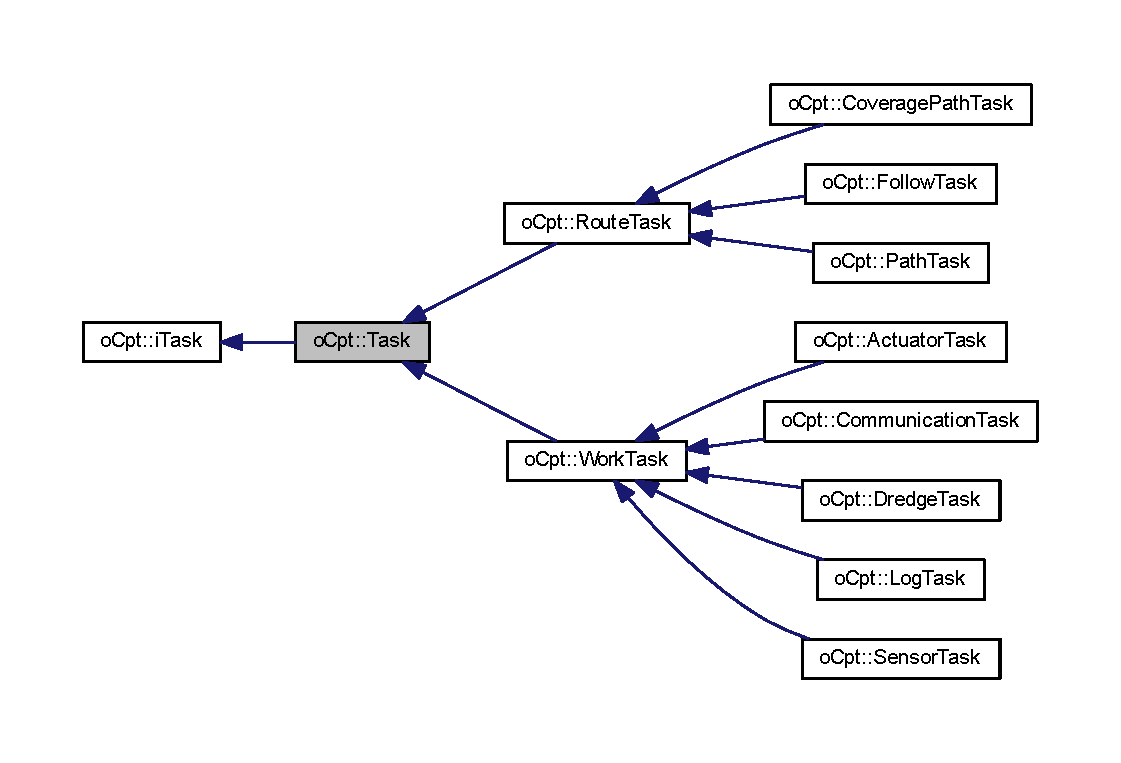
\includegraphics[width=350pt]{classo_cpt_1_1_task__inherit__graph}
\end{center}
\end{figure}


Collaboration diagram for o\+Cpt\+:\+:Task\+:\nopagebreak
\begin{figure}[H]
\begin{center}
\leavevmode
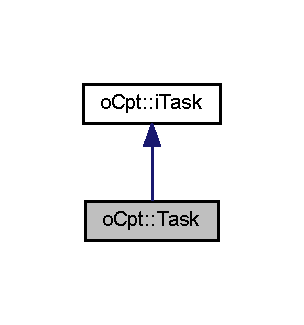
\includegraphics[width=146pt]{classo_cpt_1_1_task__coll__graph}
\end{center}
\end{figure}
\subsection*{Public Member Functions}
\begin{DoxyCompactItemize}
\item 
\hyperlink{classo_cpt_1_1_task_a814069aa4c458d09807eb78937702521}{Task} (\hyperlink{classo_cpt_1_1i_vessel_a43711a596f3bdfd0ca732ed3901edc97}{Vessel\+::ptr} vessel, bool concurrent=false)
\item 
virtual \hyperlink{classo_cpt_1_1_task_a95accf06842f78630e44190c15d6fca4}{$\sim$\+Task} ()
\item 
virtual void \hyperlink{classo_cpt_1_1_task_a8acd8d2125df0aef37eb1ebf0e3e49c8}{start} ()
\item 
virtual \hyperlink{classo_cpt_1_1i_task_1_1_status_aaf766c58d038e2defc3de2dddb92d1eb}{i\+Task\+::\+Status\+::ptr} \hyperlink{classo_cpt_1_1_task_a724445e158919a4b5644d8eef9f7c754}{status} ()
\item 
virtual void \hyperlink{classo_cpt_1_1_task_a62b4f1bbc1cf24434d2a2130162507f7}{stop} ()
\end{DoxyCompactItemize}
\subsection*{Protected Attributes}
\begin{DoxyCompactItemize}
\item 
\hyperlink{classo_cpt_1_1i_task_1_1_status_aaf766c58d038e2defc3de2dddb92d1eb}{i\+Task\+::\+Status\+::ptr} \hyperlink{classo_cpt_1_1_task_a51a0e1718a13e6d59af76511e6473743}{\+\_\+status}
\begin{DoxyCompactList}\small\item\em a boost share\+\_\+ptr to the status of a task \end{DoxyCompactList}\item 
\hyperlink{classo_cpt_1_1i_task_a10d8726eb8957c2c305f468cf15b9f11}{Type\+Of} \hyperlink{classo_cpt_1_1_task_ac4073446fdd30a1f2296da6b6fcaf802}{\+\_\+typeof}
\begin{DoxyCompactList}\small\item\em Indicating the type of a task. \end{DoxyCompactList}\end{DoxyCompactItemize}
\subsection*{Additional Inherited Members}


\subsection{Detailed Description}
The Base \hyperlink{classo_cpt_1_1_task}{Task} class 

Definition at line 111 of file Task.\+h.



\subsection{Constructor \& Destructor Documentation}
\hypertarget{classo_cpt_1_1_task_a814069aa4c458d09807eb78937702521}{}\label{classo_cpt_1_1_task_a814069aa4c458d09807eb78937702521} 
\index{o\+Cpt\+::\+Task@{o\+Cpt\+::\+Task}!Task@{Task}}
\index{Task@{Task}!o\+Cpt\+::\+Task@{o\+Cpt\+::\+Task}}
\subsubsection{\texorpdfstring{Task()}{Task()}}
{\footnotesize\ttfamily o\+Cpt\+::\+Task\+::\+Task (\begin{DoxyParamCaption}\item[{\hyperlink{classo_cpt_1_1i_vessel_a43711a596f3bdfd0ca732ed3901edc97}{Vessel\+::ptr}}]{vessel,  }\item[{bool}]{concurrent = {\ttfamily false} }\end{DoxyParamCaption})}

The contructor \begin{DoxyReturn}{Returns}

\end{DoxyReturn}


Definition at line 25 of file Task.\+cpp.



References \+\_\+status.

\hypertarget{classo_cpt_1_1_task_a95accf06842f78630e44190c15d6fca4}{}\label{classo_cpt_1_1_task_a95accf06842f78630e44190c15d6fca4} 
\index{o\+Cpt\+::\+Task@{o\+Cpt\+::\+Task}!````~Task@{$\sim$\+Task}}
\index{````~Task@{$\sim$\+Task}!o\+Cpt\+::\+Task@{o\+Cpt\+::\+Task}}
\subsubsection{\texorpdfstring{$\sim$\+Task()}{~Task()}}
{\footnotesize\ttfamily o\+Cpt\+::\+Task\+::$\sim$\+Task (\begin{DoxyParamCaption}{ }\end{DoxyParamCaption})\hspace{0.3cm}{\ttfamily [virtual]}}

The deconstructor 

Definition at line 29 of file Task.\+cpp.



\subsection{Member Function Documentation}
\hypertarget{classo_cpt_1_1_task_a8acd8d2125df0aef37eb1ebf0e3e49c8}{}\label{classo_cpt_1_1_task_a8acd8d2125df0aef37eb1ebf0e3e49c8} 
\index{o\+Cpt\+::\+Task@{o\+Cpt\+::\+Task}!start@{start}}
\index{start@{start}!o\+Cpt\+::\+Task@{o\+Cpt\+::\+Task}}
\subsubsection{\texorpdfstring{start()}{start()}}
{\footnotesize\ttfamily void o\+Cpt\+::\+Task\+::start (\begin{DoxyParamCaption}{ }\end{DoxyParamCaption})\hspace{0.3cm}{\ttfamily [virtual]}}

The start command for a task 

Implements \hyperlink{classo_cpt_1_1i_task_aedd48e3c4df48aaae0738ce3863e222f}{o\+Cpt\+::i\+Task}.



Definition at line 31 of file Task.\+cpp.



References o\+Cpt\+::i\+Task\+::\+Work.

\hypertarget{classo_cpt_1_1_task_a724445e158919a4b5644d8eef9f7c754}{}\label{classo_cpt_1_1_task_a724445e158919a4b5644d8eef9f7c754} 
\index{o\+Cpt\+::\+Task@{o\+Cpt\+::\+Task}!status@{status}}
\index{status@{status}!o\+Cpt\+::\+Task@{o\+Cpt\+::\+Task}}
\subsubsection{\texorpdfstring{status()}{status()}}
{\footnotesize\ttfamily \hyperlink{classo_cpt_1_1i_task_1_1_status_aaf766c58d038e2defc3de2dddb92d1eb}{i\+Task\+::\+Status\+::ptr} o\+Cpt\+::\+Task\+::status (\begin{DoxyParamCaption}{ }\end{DoxyParamCaption})\hspace{0.3cm}{\ttfamily [virtual]}}

Retrieves the Status of a task \begin{DoxyReturn}{Returns}
Boost shared\+\_\+ptr of the task status 
\end{DoxyReturn}


Implements \hyperlink{classo_cpt_1_1i_task_a8d6126b2e337a0ab39fdef1d8d7b73b9}{o\+Cpt\+::i\+Task}.



Definition at line 37 of file Task.\+cpp.



References \+\_\+status.

\hypertarget{classo_cpt_1_1_task_a62b4f1bbc1cf24434d2a2130162507f7}{}\label{classo_cpt_1_1_task_a62b4f1bbc1cf24434d2a2130162507f7} 
\index{o\+Cpt\+::\+Task@{o\+Cpt\+::\+Task}!stop@{stop}}
\index{stop@{stop}!o\+Cpt\+::\+Task@{o\+Cpt\+::\+Task}}
\subsubsection{\texorpdfstring{stop()}{stop()}}
{\footnotesize\ttfamily void o\+Cpt\+::\+Task\+::stop (\begin{DoxyParamCaption}{ }\end{DoxyParamCaption})\hspace{0.3cm}{\ttfamily [virtual]}}

The stop command for a task 

Implements \hyperlink{classo_cpt_1_1i_task_aedb88813b16914598dee9561813e56e8}{o\+Cpt\+::i\+Task}.



Definition at line 39 of file Task.\+cpp.



\subsection{Member Data Documentation}
\hypertarget{classo_cpt_1_1_task_a51a0e1718a13e6d59af76511e6473743}{}\label{classo_cpt_1_1_task_a51a0e1718a13e6d59af76511e6473743} 
\index{o\+Cpt\+::\+Task@{o\+Cpt\+::\+Task}!\+\_\+status@{\+\_\+status}}
\index{\+\_\+status@{\+\_\+status}!o\+Cpt\+::\+Task@{o\+Cpt\+::\+Task}}
\subsubsection{\texorpdfstring{\+\_\+status}{\_status}}
{\footnotesize\ttfamily \hyperlink{classo_cpt_1_1i_task_1_1_status_aaf766c58d038e2defc3de2dddb92d1eb}{i\+Task\+::\+Status\+::ptr} o\+Cpt\+::\+Task\+::\+\_\+status\hspace{0.3cm}{\ttfamily [protected]}}



a boost share\+\_\+ptr to the status of a task 



Definition at line 141 of file Task.\+h.



Referenced by status(), and Task().

\hypertarget{classo_cpt_1_1_task_ac4073446fdd30a1f2296da6b6fcaf802}{}\label{classo_cpt_1_1_task_ac4073446fdd30a1f2296da6b6fcaf802} 
\index{o\+Cpt\+::\+Task@{o\+Cpt\+::\+Task}!\+\_\+typeof@{\+\_\+typeof}}
\index{\+\_\+typeof@{\+\_\+typeof}!o\+Cpt\+::\+Task@{o\+Cpt\+::\+Task}}
\subsubsection{\texorpdfstring{\+\_\+typeof}{\_typeof}}
{\footnotesize\ttfamily \hyperlink{classo_cpt_1_1i_task_a10d8726eb8957c2c305f468cf15b9f11}{Type\+Of} o\+Cpt\+::\+Task\+::\+\_\+typeof\hspace{0.3cm}{\ttfamily [protected]}}



Indicating the type of a task. 



Definition at line 142 of file Task.\+h.



Referenced by o\+Cpt\+::\+Route\+Task\+::\+Route\+Task(), and o\+Cpt\+::\+Work\+Task\+::\+Work\+Task().



The documentation for this class was generated from the following files\+:\begin{DoxyCompactItemize}
\item 
include/\+Core/\hyperlink{_task_8h}{Task.\+h}\item 
src/\+Core/\hyperlink{_task_8cpp}{Task.\+cpp}\end{DoxyCompactItemize}

\hypertarget{classo_cpt_1_1_work_task}{}\section{o\+Cpt\+:\+:Work\+Task Class Reference}
\label{classo_cpt_1_1_work_task}\index{o\+Cpt\+::\+Work\+Task@{o\+Cpt\+::\+Work\+Task}}


{\ttfamily \#include $<$Task.\+h$>$}

Inheritance diagram for o\+Cpt\+:\+:Work\+Task\+:\begin{figure}[H]
\begin{center}
\leavevmode
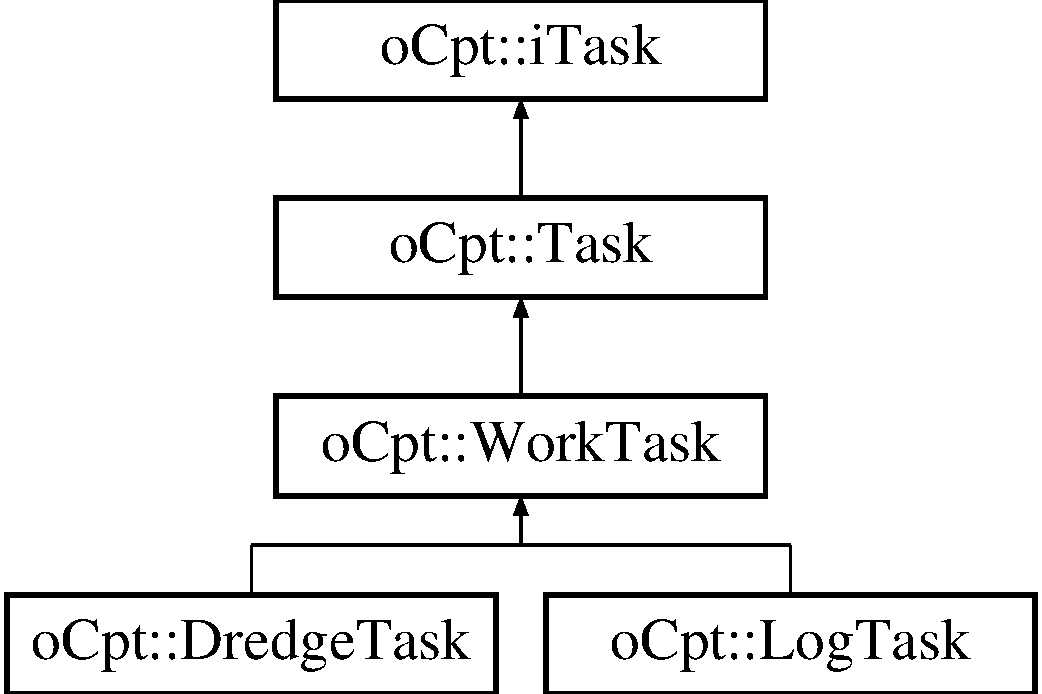
\includegraphics[height=4.000000cm]{classo_cpt_1_1_work_task}
\end{center}
\end{figure}
\subsection*{Public Member Functions}
\begin{DoxyCompactItemize}
\item 
\hyperlink{classo_cpt_1_1_work_task_ac150cf3b1094a9274dcef3b28a385315}{Work\+Task} ()
\item 
virtual \hyperlink{classo_cpt_1_1_work_task_a9158f1f64ab798531258775607377383}{$\sim$\+Work\+Task} ()
\end{DoxyCompactItemize}
\subsection*{Additional Inherited Members}


\subsection{Detailed Description}
An object representing work related tasks 

\subsection{Constructor \& Destructor Documentation}
\index{o\+Cpt\+::\+Work\+Task@{o\+Cpt\+::\+Work\+Task}!Work\+Task@{Work\+Task}}
\index{Work\+Task@{Work\+Task}!o\+Cpt\+::\+Work\+Task@{o\+Cpt\+::\+Work\+Task}}
\subsubsection[{\texorpdfstring{Work\+Task()}{WorkTask()}}]{\setlength{\rightskip}{0pt plus 5cm}o\+Cpt\+::\+Work\+Task\+::\+Work\+Task (
\begin{DoxyParamCaption}
{}
\end{DoxyParamCaption}
)}\hypertarget{classo_cpt_1_1_work_task_ac150cf3b1094a9274dcef3b28a385315}{}\label{classo_cpt_1_1_work_task_ac150cf3b1094a9274dcef3b28a385315}
Constructor of the interface \begin{DoxyReturn}{Returns}

\end{DoxyReturn}
\index{o\+Cpt\+::\+Work\+Task@{o\+Cpt\+::\+Work\+Task}!````~Work\+Task@{$\sim$\+Work\+Task}}
\index{````~Work\+Task@{$\sim$\+Work\+Task}!o\+Cpt\+::\+Work\+Task@{o\+Cpt\+::\+Work\+Task}}
\subsubsection[{\texorpdfstring{$\sim$\+Work\+Task()}{~WorkTask()}}]{\setlength{\rightskip}{0pt plus 5cm}o\+Cpt\+::\+Work\+Task\+::$\sim$\+Work\+Task (
\begin{DoxyParamCaption}
{}
\end{DoxyParamCaption}
)\hspace{0.3cm}{\ttfamily [virtual]}}\hypertarget{classo_cpt_1_1_work_task_a9158f1f64ab798531258775607377383}{}\label{classo_cpt_1_1_work_task_a9158f1f64ab798531258775607377383}
The deconstructor 

The documentation for this class was generated from the following files\+:\begin{DoxyCompactItemize}
\item 
include/\hyperlink{_task_8h}{Task.\+h}\item 
src/\hyperlink{_task_8cpp}{Task.\+cpp}\end{DoxyCompactItemize}

\chapter{File Documentation}
\hypertarget{_task_8h}{}\section{/projects/mti/oh\+Captain/oh\+Captain/include/\+Core/\+Task.h File Reference}
\label{_task_8h}\index{/projects/mti/oh\+Captain/oh\+Captain/include/\+Core/\+Task.\+h@{/projects/mti/oh\+Captain/oh\+Captain/include/\+Core/\+Task.\+h}}
{\ttfamily \#include $<$boost/shared\+\_\+ptr.\+hpp$>$}\newline
{\ttfamily \#include $<$list$>$}\newline
{\ttfamily \#include \char`\"{}Vessel.\+h\char`\"{}}\newline
Include dependency graph for Task.\+h\+:
\nopagebreak
\begin{figure}[H]
\begin{center}
\leavevmode
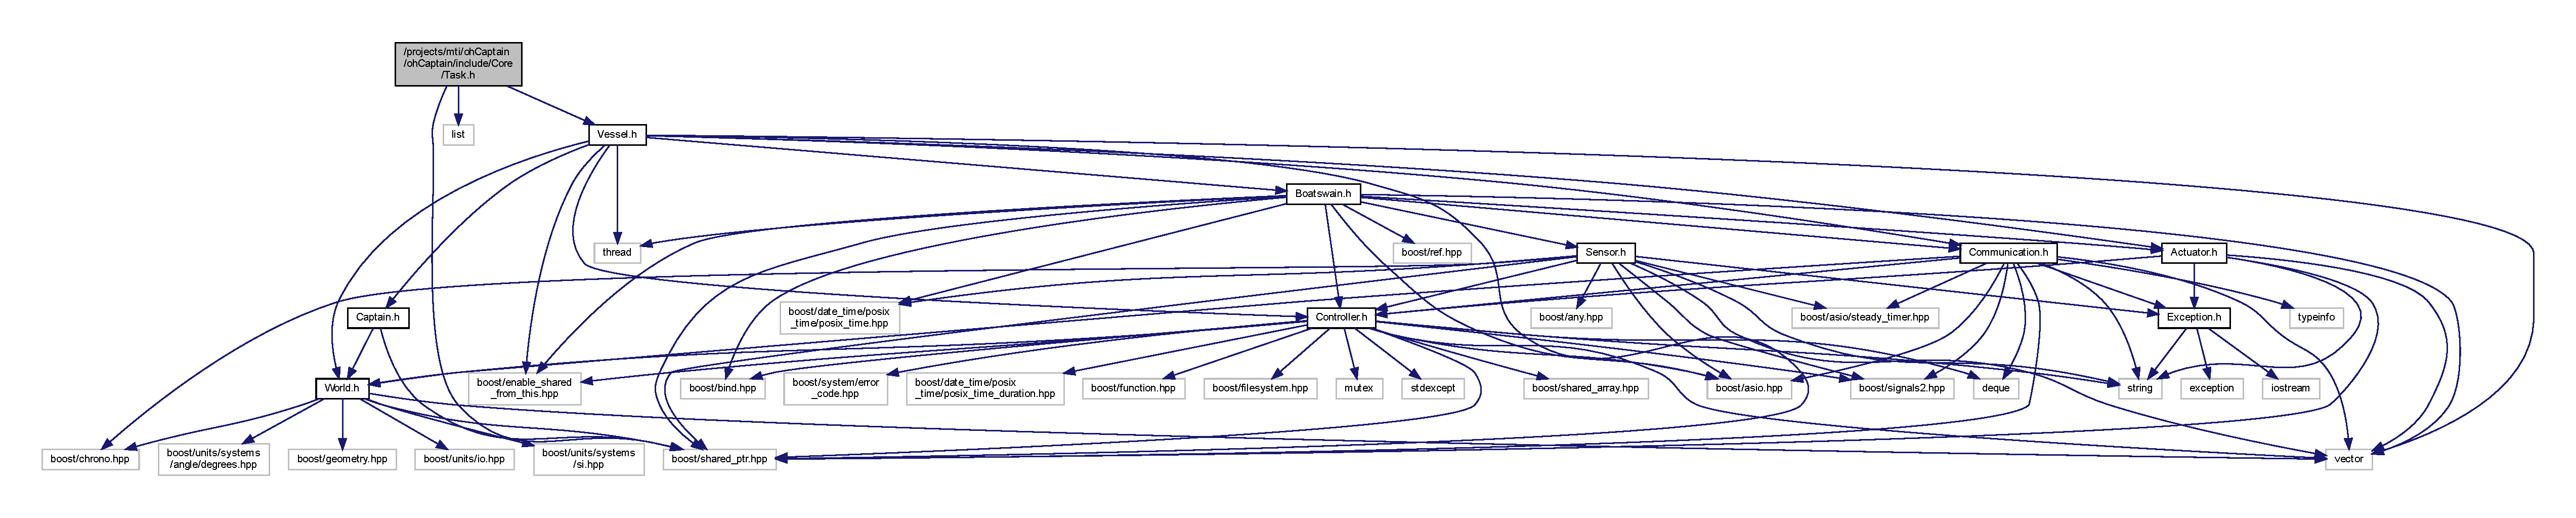
\includegraphics[width=350pt]{_task_8h__incl}
\end{center}
\end{figure}
This graph shows which files directly or indirectly include this file\+:
\nopagebreak
\begin{figure}[H]
\begin{center}
\leavevmode
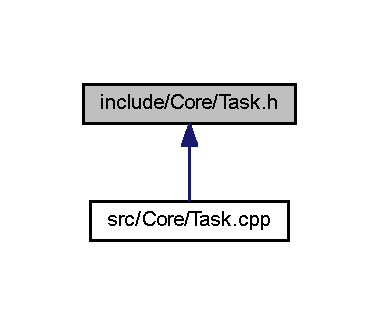
\includegraphics[width=226pt]{_task_8h__dep__incl}
\end{center}
\end{figure}
\subsection*{Classes}
\begin{DoxyCompactItemize}
\item 
class \hyperlink{classo_cpt_1_1i_task}{o\+Cpt\+::i\+Task}
\begin{DoxyCompactList}\small\item\em \hyperlink{classo_cpt_1_1_task}{Task} interface, all tasks need to adhere to this structure. \end{DoxyCompactList}\item 
class \hyperlink{classo_cpt_1_1i_task_1_1_status}{o\+Cpt\+::i\+Task\+::\+Status}
\item 
class \hyperlink{classo_cpt_1_1_task}{o\+Cpt\+::\+Task}
\item 
class \hyperlink{classo_cpt_1_1_route_task}{o\+Cpt\+::\+Route\+Task}
\item 
class \hyperlink{classo_cpt_1_1_work_task}{o\+Cpt\+::\+Work\+Task}
\item 
class \hyperlink{classo_cpt_1_1_coverage_path_task}{o\+Cpt\+::\+Coverage\+Path\+Task}
\begin{DoxyCompactList}\small\item\em An object representing a coverage path task. \end{DoxyCompactList}\item 
class \hyperlink{classo_cpt_1_1_follow_task}{o\+Cpt\+::\+Follow\+Task}
\begin{DoxyCompactList}\small\item\em An object representing a follow the target task. \end{DoxyCompactList}\item 
class \hyperlink{classo_cpt_1_1_path_task}{o\+Cpt\+::\+Path\+Task}
\begin{DoxyCompactList}\small\item\em An object representing a normal A to B type of path planning. \end{DoxyCompactList}\item 
class \hyperlink{classo_cpt_1_1_log_task}{o\+Cpt\+::\+Log\+Task}
\begin{DoxyCompactList}\small\item\em An Object representing a data logging task. \end{DoxyCompactList}\item 
class \hyperlink{classo_cpt_1_1_dredge_task}{o\+Cpt\+::\+Dredge\+Task}
\begin{DoxyCompactList}\small\item\em An Object representing a dredging task. \end{DoxyCompactList}\item 
class \hyperlink{classo_cpt_1_1_sensor_task}{o\+Cpt\+::\+Sensor\+Task}
\item 
class \hyperlink{classo_cpt_1_1_actuator_task}{o\+Cpt\+::\+Actuator\+Task}
\item 
class \hyperlink{classo_cpt_1_1_communication_task}{o\+Cpt\+::\+Communication\+Task}
\end{DoxyCompactItemize}
\subsection*{Namespaces}
\begin{DoxyCompactItemize}
\item 
 \hyperlink{namespaceo_cpt}{o\+Cpt}
\end{DoxyCompactItemize}

\hypertarget{_task_8cpp}{}\section{src/\+Core/\+Task.cpp File Reference}
\label{_task_8cpp}\index{src/\+Core/\+Task.\+cpp@{src/\+Core/\+Task.\+cpp}}
{\ttfamily \#include \char`\"{}../../include/\+Core/\+Task.\+h\char`\"{}}\newline
Include dependency graph for Task.\+cpp\+:
\nopagebreak
\begin{figure}[H]
\begin{center}
\leavevmode
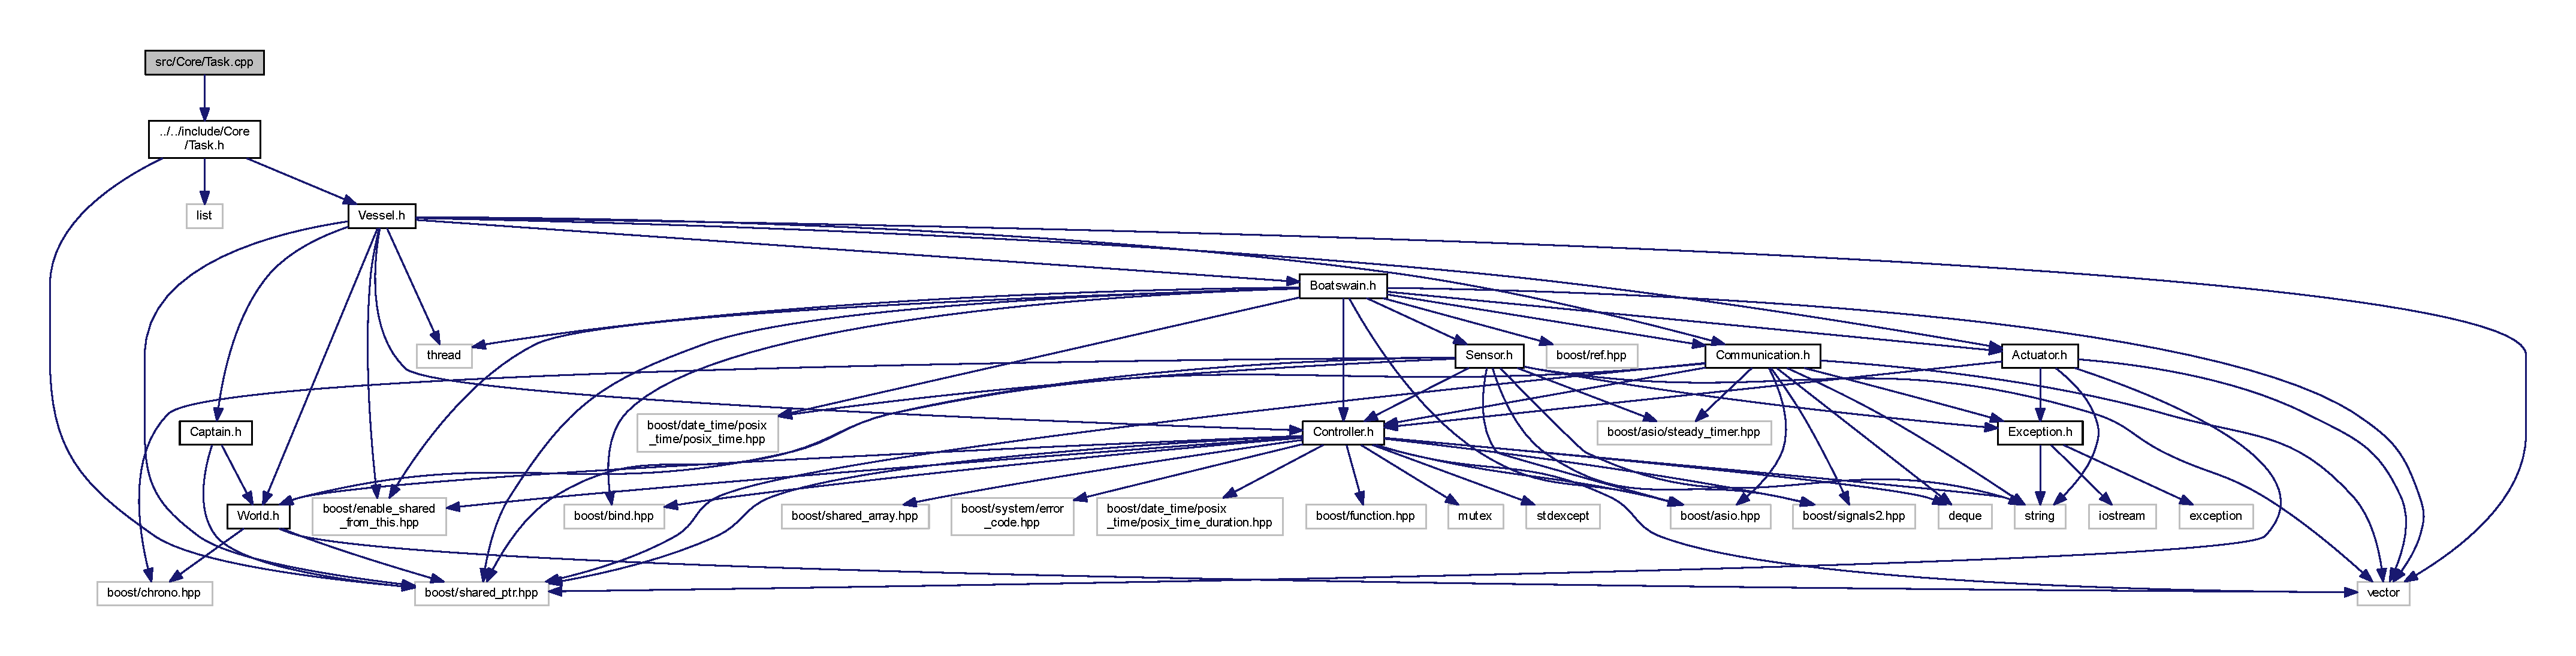
\includegraphics[width=350pt]{_task_8cpp__incl}
\end{center}
\end{figure}
\subsection*{Namespaces}
\begin{DoxyCompactItemize}
\item 
 \hyperlink{namespaceo_cpt}{o\+Cpt}
\end{DoxyCompactItemize}

%--- End generated contents ---

% Index
\backmatter
\newpage
\phantomsection
\clearemptydoublepage
\addcontentsline{toc}{chapter}{Index}
\printindex

\end{document}
